\documentclass{article}
\usepackage{graphicx}
\usepackage{subcaption}
\usepackage{amsmath}
\usepackage{cite}  % Optional for better citation management
\usepackage{placeins}

\title{Weekly meeting notes}
\author{Eugenio Pescimoro }

\begin{document}

\maketitle

\section{Introduction}
The aim of these notes is to describe the numerical modelling of solute transport and diffusion through fractured porous media using a random walk approach.

\FloatBarrier  % Prevents figures from floating past this point
\section{Diffusion in fractures}
The drifting term..

\FloatBarrier  % Prevents figures from floating past this point
\section{Code verification}
As a first step for ensuring the reliability of a solute transport simulation code it is essential to verify that the solutions of numerical experiments and analytical study coincide. For this purpose we compare the analytical solutions from three different transport problems against the numerically generated results, namely:
\begin{itemize}
    \item spatial distribution of the concentration at a given time for a solute that is displaced through an infinite bi-dimensional domain with horizontal impenetrable boundaries and initial one-dimensional vertical location;
    \item probability density function of a breakthrough curve for a solute which is displaced through a semi-infinite domain where particles' arriving times are recorded on a vertical absorbing control plane;
    \item the survived particle in time curve for a solute subject to an exponential degradation process. 
\end{itemize}

\subsection{Infinite domain}
In this test (Figure \ref{fig:Infinite}) we release $10^4$ particles in a horizontally infinite domain. Reflecting properties are assigned to the upper and lower horizontal boundaries and the simulation is run for $10^3$ time steps. After $10^2$ time steps the spatial distribution of the solute is recorded and compared against the analytical solution at the same time, namely:
\begin{equation}
    c(x) = \frac{e^{-\frac{x^2}{4 D t}}}{\sqrt{4 \pi D t}}.
\end{equation}

\begin{figure}[htbp]
    \centering
    \begin{subfigure}[b]{0.3\textwidth}
        \centering
        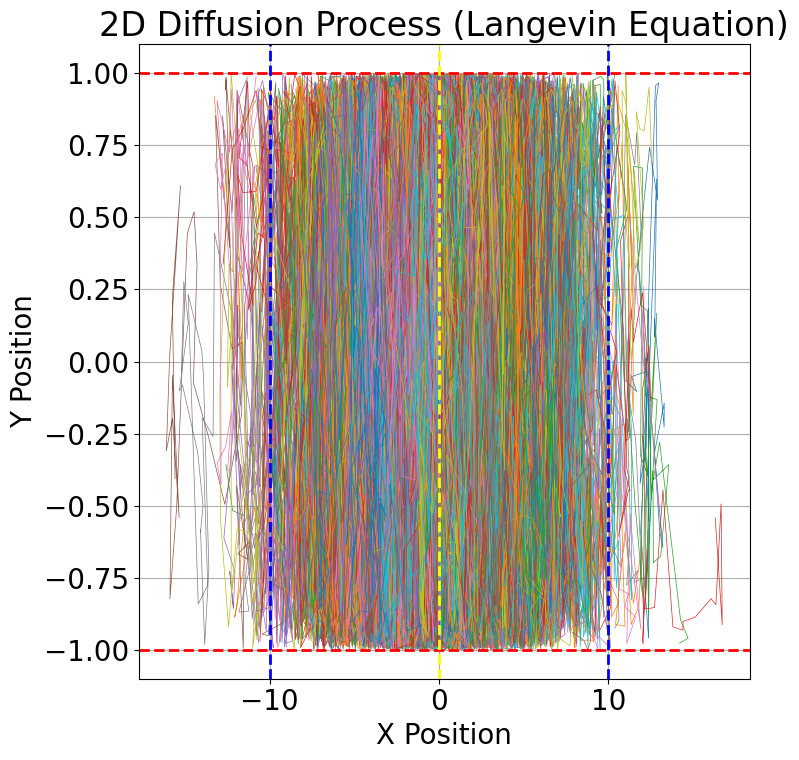
\includegraphics[width=\textwidth]{images/trajectoriesInfinite.png} % Replace with your image path
        \caption{Trajectories of 1e4 particles during 1e3 time steps}
        \label{fig:subplotTrInf}
    \end{subfigure}
    \hfill
    \begin{subfigure}[b]{0.3\textwidth}
        \centering
        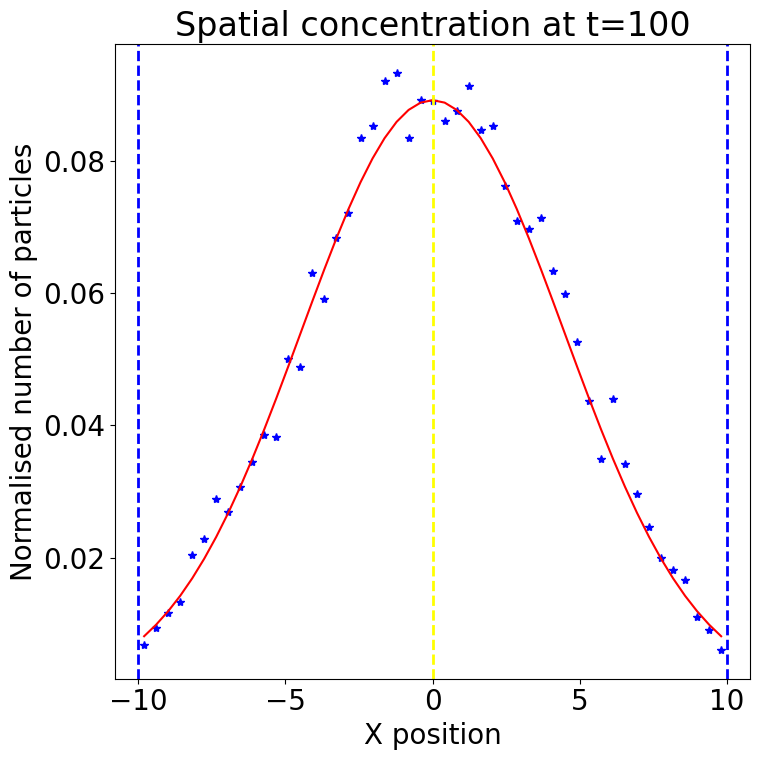
\includegraphics[width=\textwidth]{images/verificationInfinite1e4.png} % Replace with your image path
        \caption{Spatial distribution of the particles at time 1e2}
        \label{fig:subplotVerInf}
    \end{subfigure}
    \hfill
    \begin{subfigure}[b]{0.3\textwidth}
        \centering
        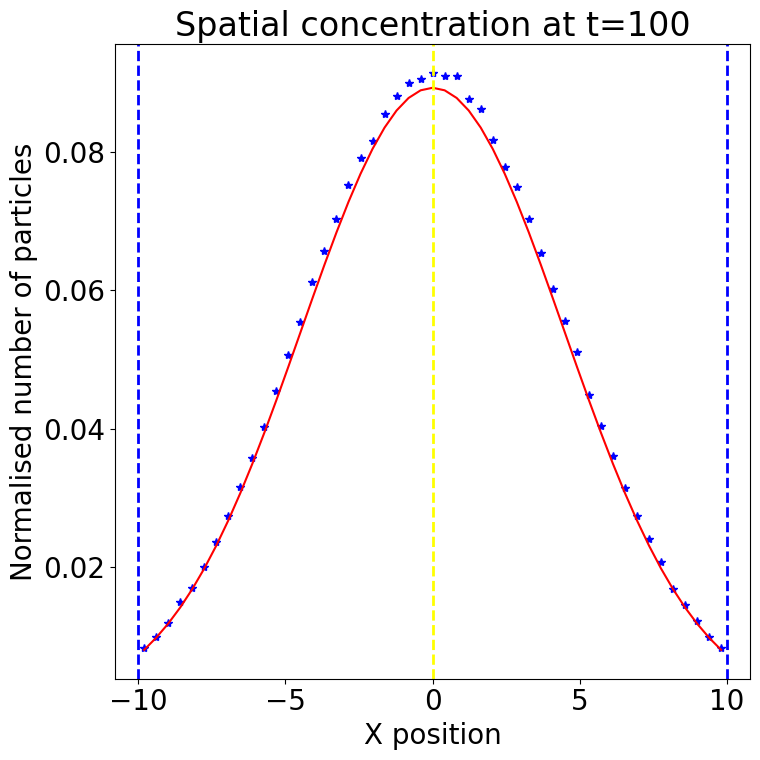
\includegraphics[width=\textwidth]{images/verificationInfinite1e6.png} % Replace with your image path
        \caption{Spatial distribution of the particles at time 1e2 with 1e5 particles}
        \label{fig:subplotVerInf1e5}
    \end{subfigure}
    \caption{Verification of the code comparing two spatial distribution of the concentration at a given time: solid blue line represents the spatial concentration from a numerical simulation while solid red line shows the analytical solution of the spatial concentration in a infinite domain at the same given time.}
    \label{fig:Infinite}
\end{figure}

\subsection{Semi-infinite domain}
In this test (Figure \ref{fig:SemiInfinite}), the arrival times of the particles are recorded on the left absorbing boundary. The spatial bins are logarithmically spaced and the number of particles per time bin is divided by the total number of particles and the width of the temporal bin. This result is compared against its analytical solution, namely:
\begin{equation}
        c(t) = \frac{x_0 e^{-\frac{x_0^2}{4 D t}}}{\sqrt{4 \pi D t^3}}
        \label{eq:SemiInfConc}
\end{equation}
where $x_0$ is the distance between the vertical plane where particle are released and the absorbing vertical plane.

\begin{figure}[htbp]
    \centering
    \begin{subfigure}[b]{0.3\textwidth}
        \centering
        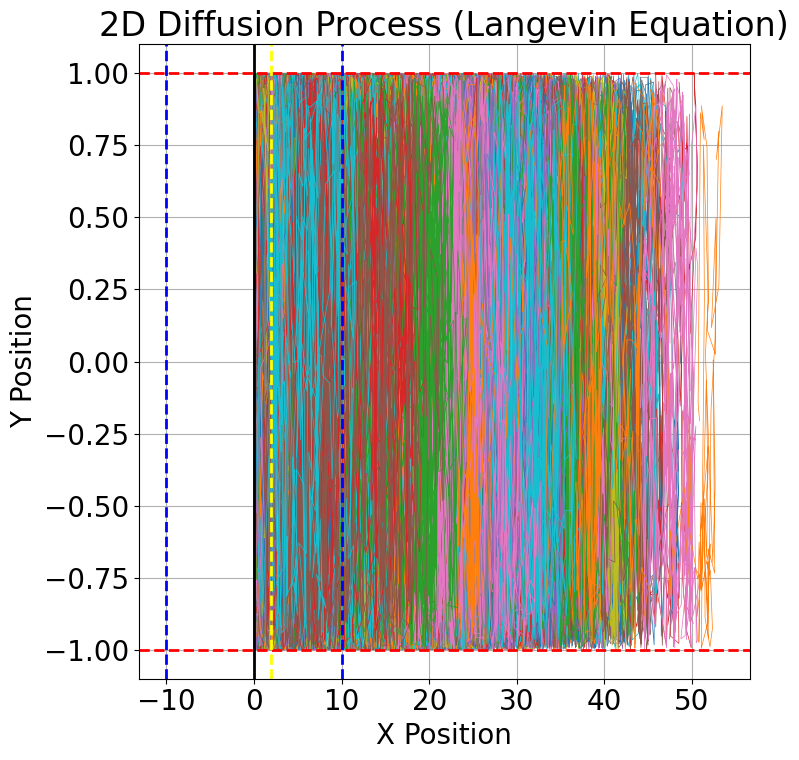
\includegraphics[width=\textwidth]{images/trajectoriesSemiInfinite.png} % Replace with your image path
        \caption{Trajectories of 1e4 particles during 1e3 time steps}
        \label{fig:subplotTrSemiInf}
    \end{subfigure}
    \hfill
    \begin{subfigure}[b]{0.3\textwidth}
        \centering
        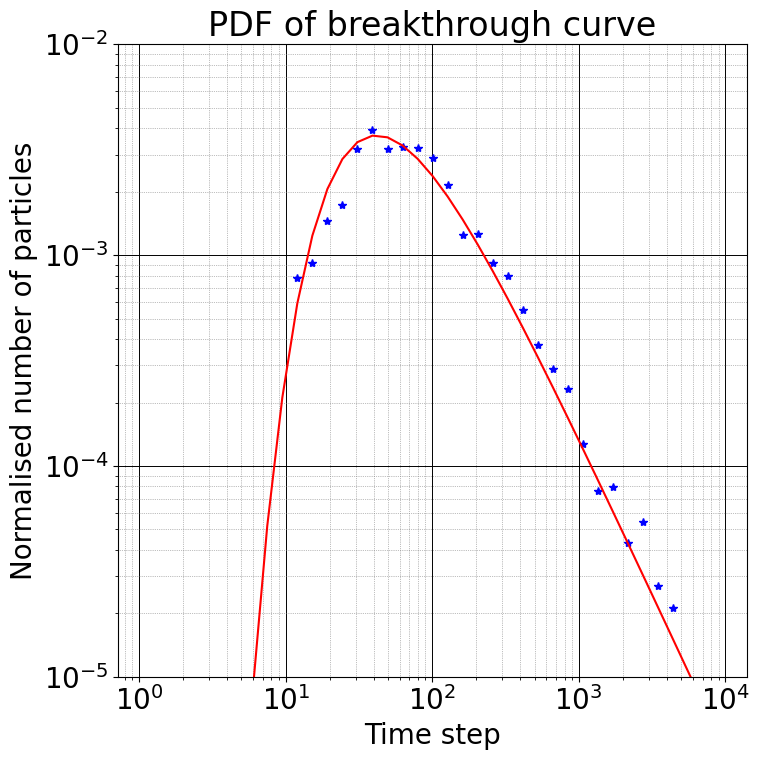
\includegraphics[width=\textwidth]{images/verificationSemi-infinite1e3.png} % Replace with your image path
        \caption{Arrival times on the left absorbing boundary}
        \label{fig:subplotVerSemiInf}
    \end{subfigure}
    \hfill
    \begin{subfigure}[b]{0.3\textwidth}
        \centering
        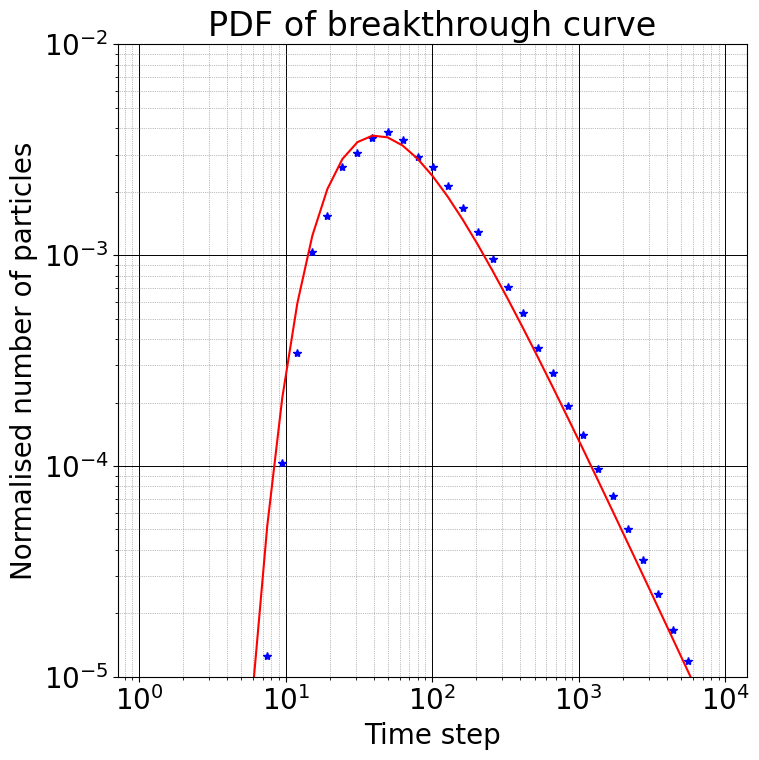
\includegraphics[width=\textwidth]{images/verificationSemi-infinite1e5.png} % Replace with your image path
        \caption{Arrival times on the left absorbing boundary with 1e4 particles, 1e4 time steps and x0=4}
        \label{fig:subplotVerSemiInfImproved}
    \end{subfigure}
    \caption{Verification of the code comparing two pdfs of the btc: blue dots represent the btc pdf from numerical simulation, solid red line is the analytical solution of the btc pdf for a semi-infinite domain}
    \label{fig:SemiInfinite}
\end{figure}

\subsection{Degradation}
This test (Figure \ref{fig:Degradation}) focuses on a horizontally infinite scenario where $10^3$ particles travel for maximum $10^3$ time steps. The upper and lower horizontal boundaries are both reflecting the particles however, some of the latter disappear due to a degradation process which follows an exponential trend:
\begin{equation}
    p_s(t) = k e^{-kt}
\end{equation}
where $p_s(t)$ is the survival probability distribution. Before the simulation, the survival probability of each particle is a random variable charaterised by the $p_s(t)$ probability distribution with values between 0 and the maximum number of time steps. After every time step, the particles' survival time is withdrawn from the simulation if its survival time is less than the time step. The degradation kinetic constant $k$ for the following simulation was assigned an arbitrary value equal to 0.01.

\begin{figure}[htbp]
    \centering
    \begin{subfigure}[b]{0.45\textwidth}
        \centering
        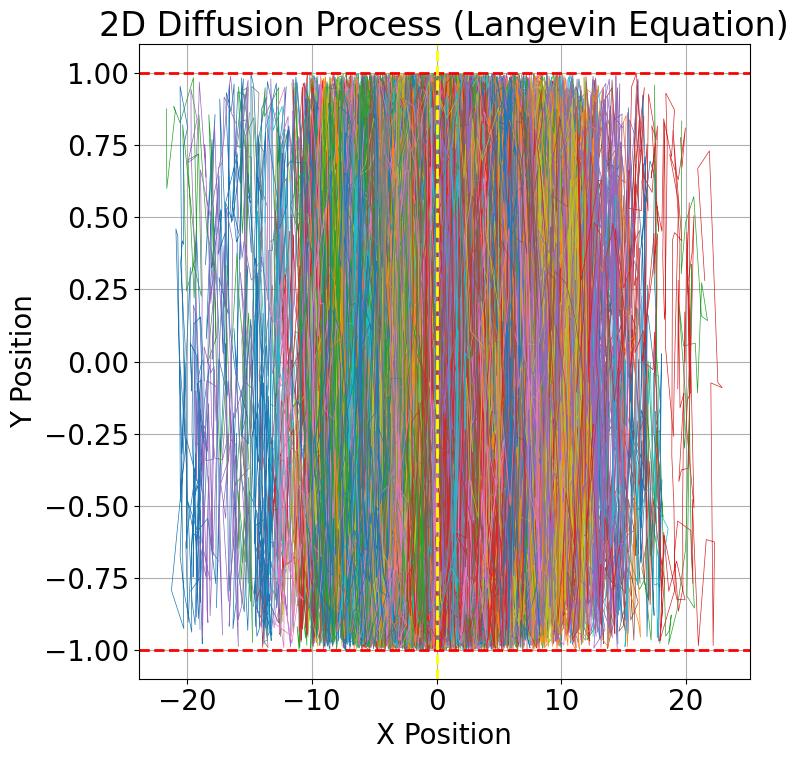
\includegraphics[width=\textwidth]{images/trajectoriesDegradation.png} % Replace with your image path
        \caption{Trajectories of 1e3 particles during 1e3 time steps with degradation}
        \label{fig:subplotTrDeg}
    \end{subfigure}
    \hfill
    \begin{subfigure}[b]{0.45\textwidth}
        \centering
        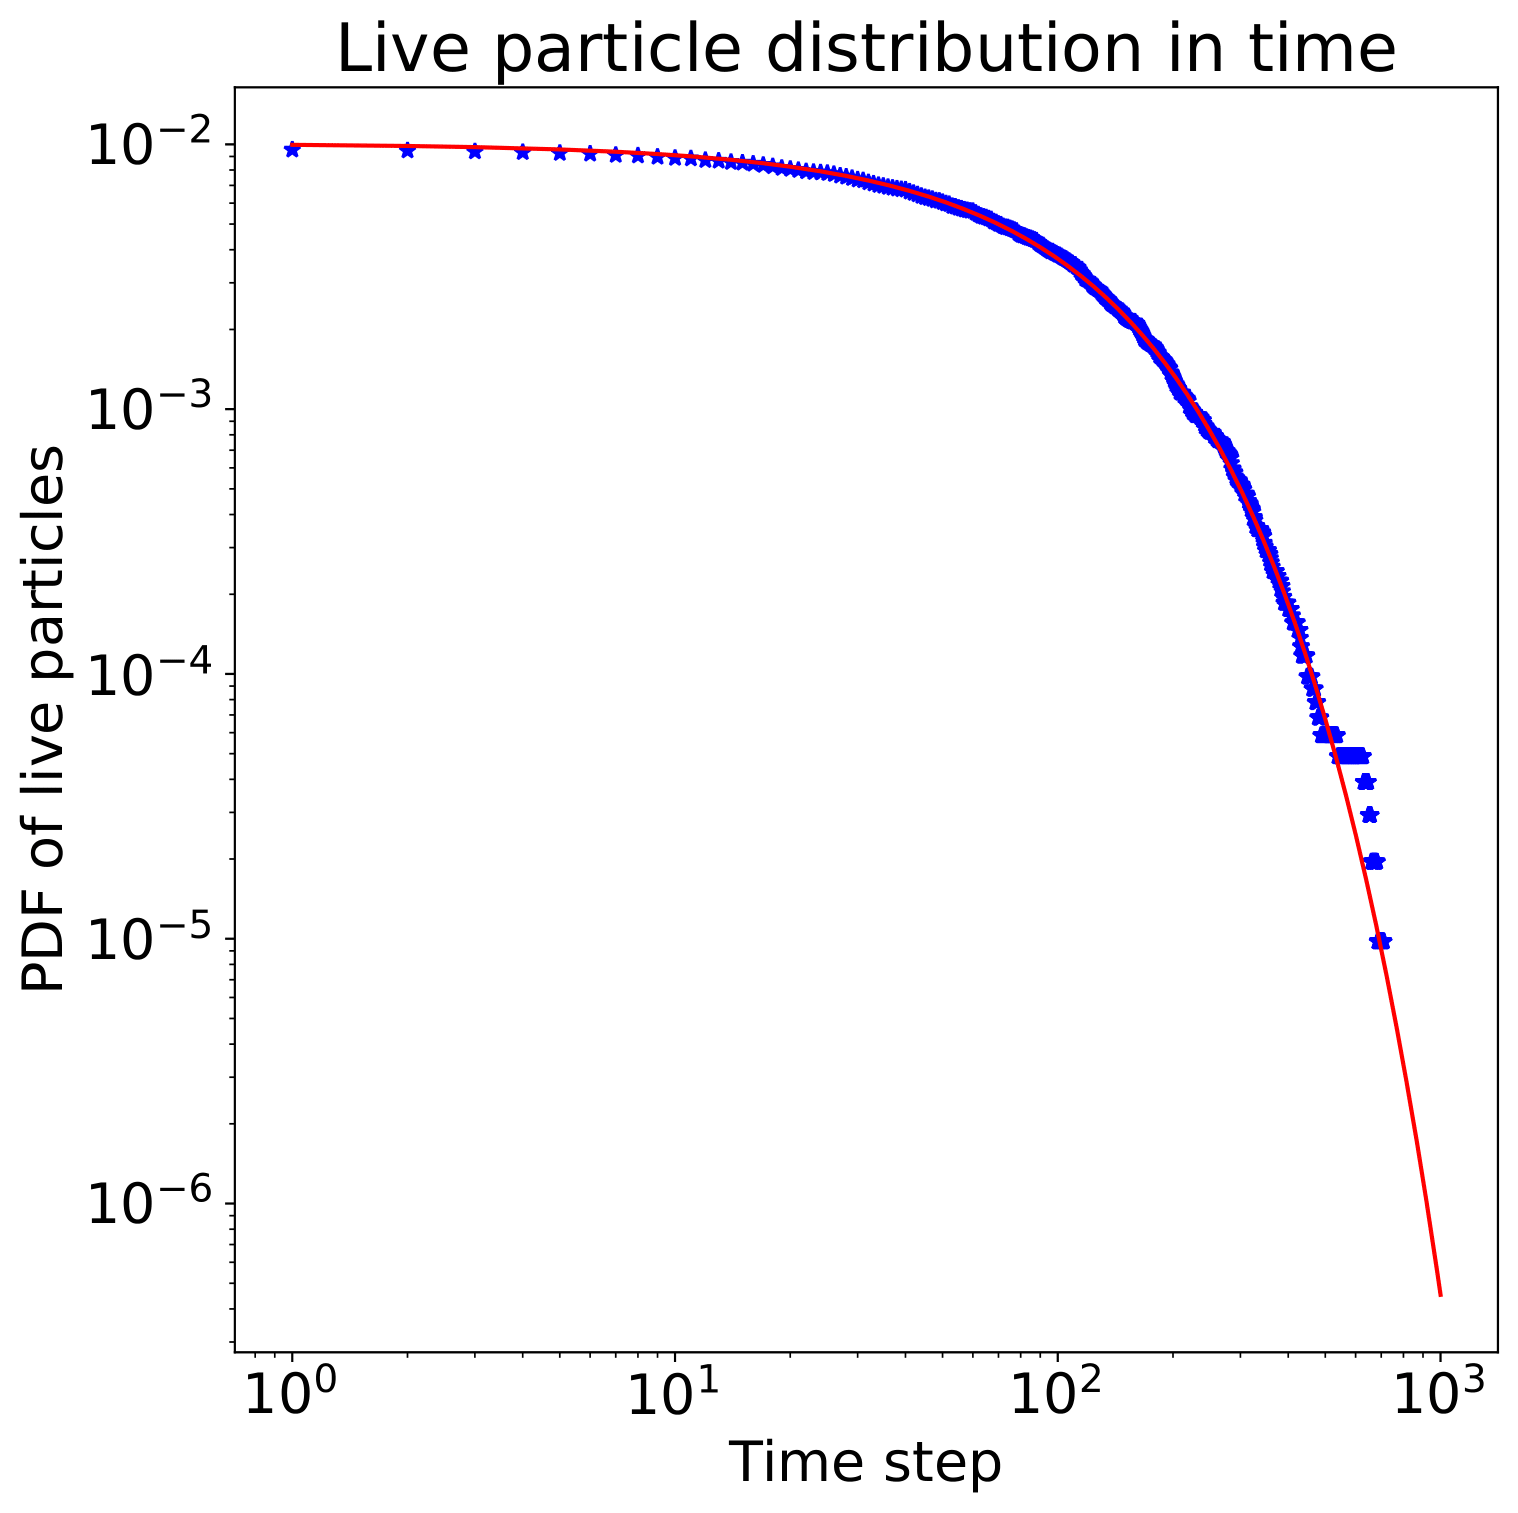
\includegraphics[width=\textwidth]{images/liveParticleInTime.png} % Replace with your image path
        \caption{PDF of survived particles in time}
        \label{fig:subplotLivePart}
    \end{subfigure}
    \caption{Verification of the code comparing two pdfs of the btc: blue dots represent the btc pdf from numerical simulation, solid red line is the analytical solution of the btc pdf}
    \label{fig:Degradation}
\end{figure}

\FloatBarrier  % Prevents figures from floating past this point
\section{Absorbing boundaries}
For the case where the particles which impact the lower and upper boundaries are absorbed, the analytical solution is not available. In the following example (Figure \ref{fig:finalPos} - Figure \ref{fig:AbsorptionInTime}), the particles which hit the boundaries have 100\% probability of being absorbed. An alternative which has been implemented in the code but is not currently shown allows to assign to the particles different absorption probability that is, the outcome of the impact of particle with the walls (either reflected or absorbed) will becomes a random variable which is drawn from a custom probability distribution.

\FloatBarrier  % Prevents figures from floating past this point
\subsection{Final positions}
The final position of $10^4$ particles after 20 steps is shown in Figure \ref{fig:finalPos}.
\begin{figure}[htbp]
    \centering
    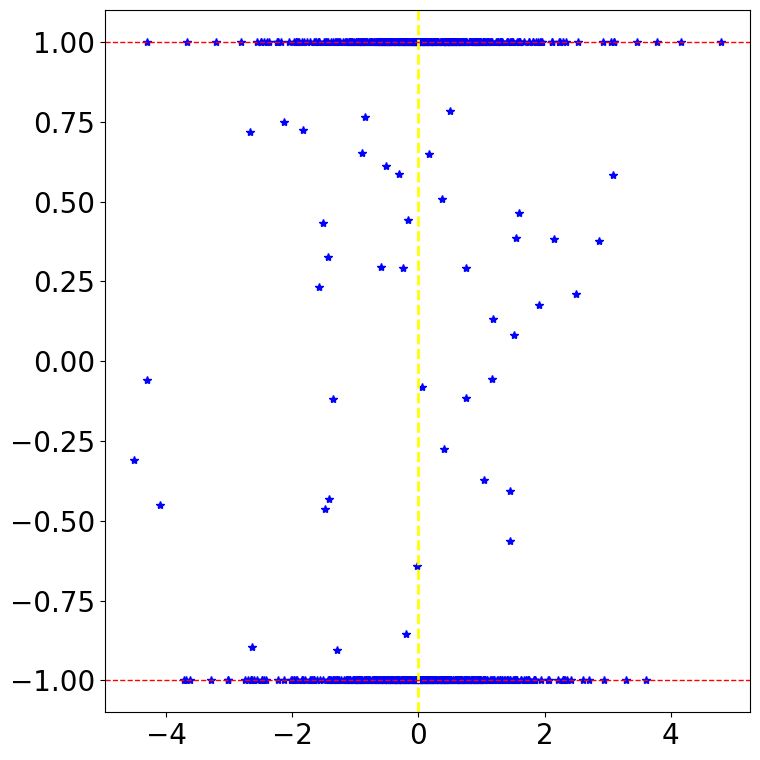
\includegraphics[width=0.5\textwidth]{images/finalPositions.png}
    \caption{Final position for 1e4 particles after 20 steps in a domain characterised by absorbing boundaries}
    \label{fig:finalPos}
\end{figure}

\FloatBarrier  % Prevents figures from floating past this point
\subsection{Cross section histograms}
Figures \ref{fig:subplotVertFinal} and \ref{fig:subplotHorFinal} show the number of particles in two different regions of space at the end of the simulation. 
\begin{figure}[htbp]
    \centering
    \begin{subfigure}[b]{0.45\textwidth}
        \centering
        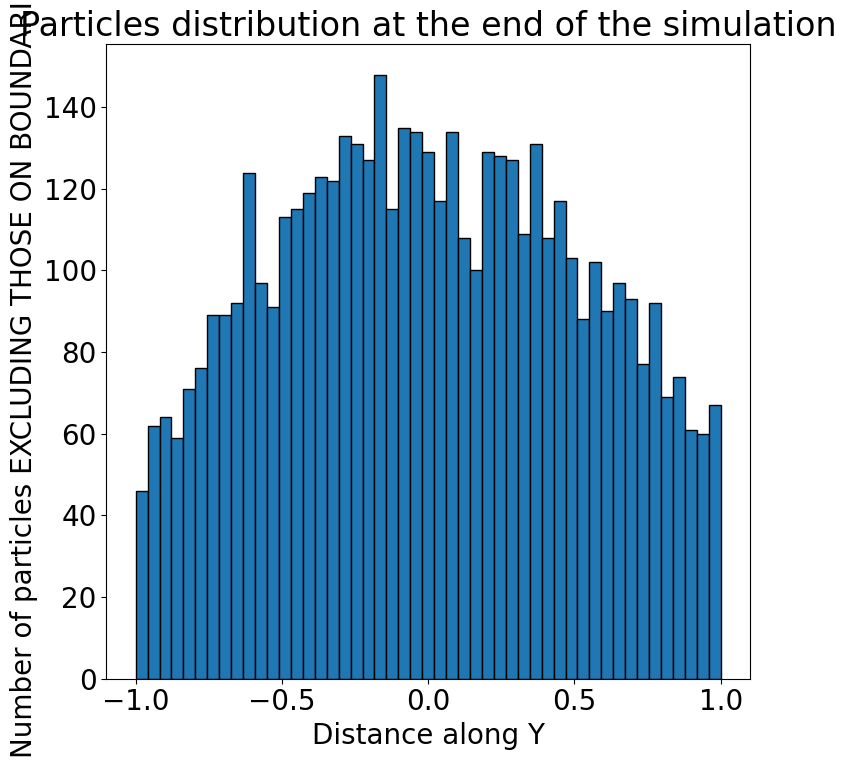
\includegraphics[width=\textwidth]{images/verticalFinalDist.png} % Replace with your image path
        \caption{Vertical distribution of particles}
        \label{fig:subplotVertFinal}
    \end{subfigure}
    \hfill
    \begin{subfigure}[b]{0.45\textwidth}
        \centering
        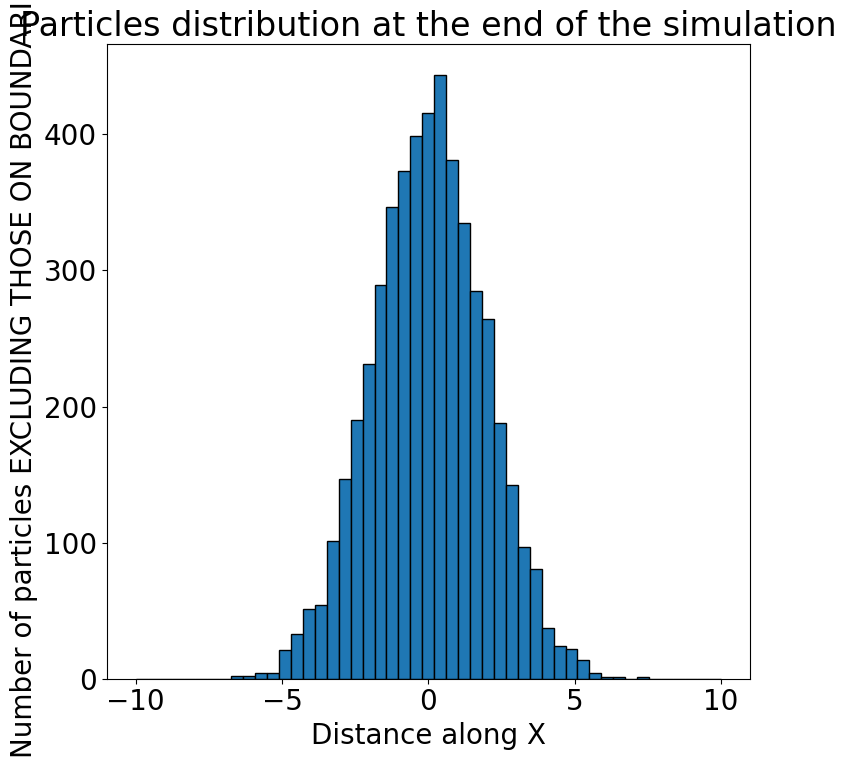
\includegraphics[width=\textwidth]{images/horizontalFinalDist.png} % Replace with your image path
        \caption{Horizontal distribution of particles}
        \label{fig:subplotHorFinal}
    \end{subfigure}
    \caption{Absorbing boundaries}
    \label{fig:Absorption}
\end{figure}

\FloatBarrier  % Prevents figures from floating past this point
\subsection{Non-adsorbed particles in time}
Figure \ref{fig:AbsorptionInTime} show the number of free particles, i.e. those that were not absorbed, throughout time. The probability for the particles to be absorbed by the boundaries of the fracture is:
\begin{equation}
    p_a = 100 \%
\end{equation}
\begin{figure}[htbp]
    \centering
    \begin{subfigure}[b]{0.45\textwidth}
        \centering
        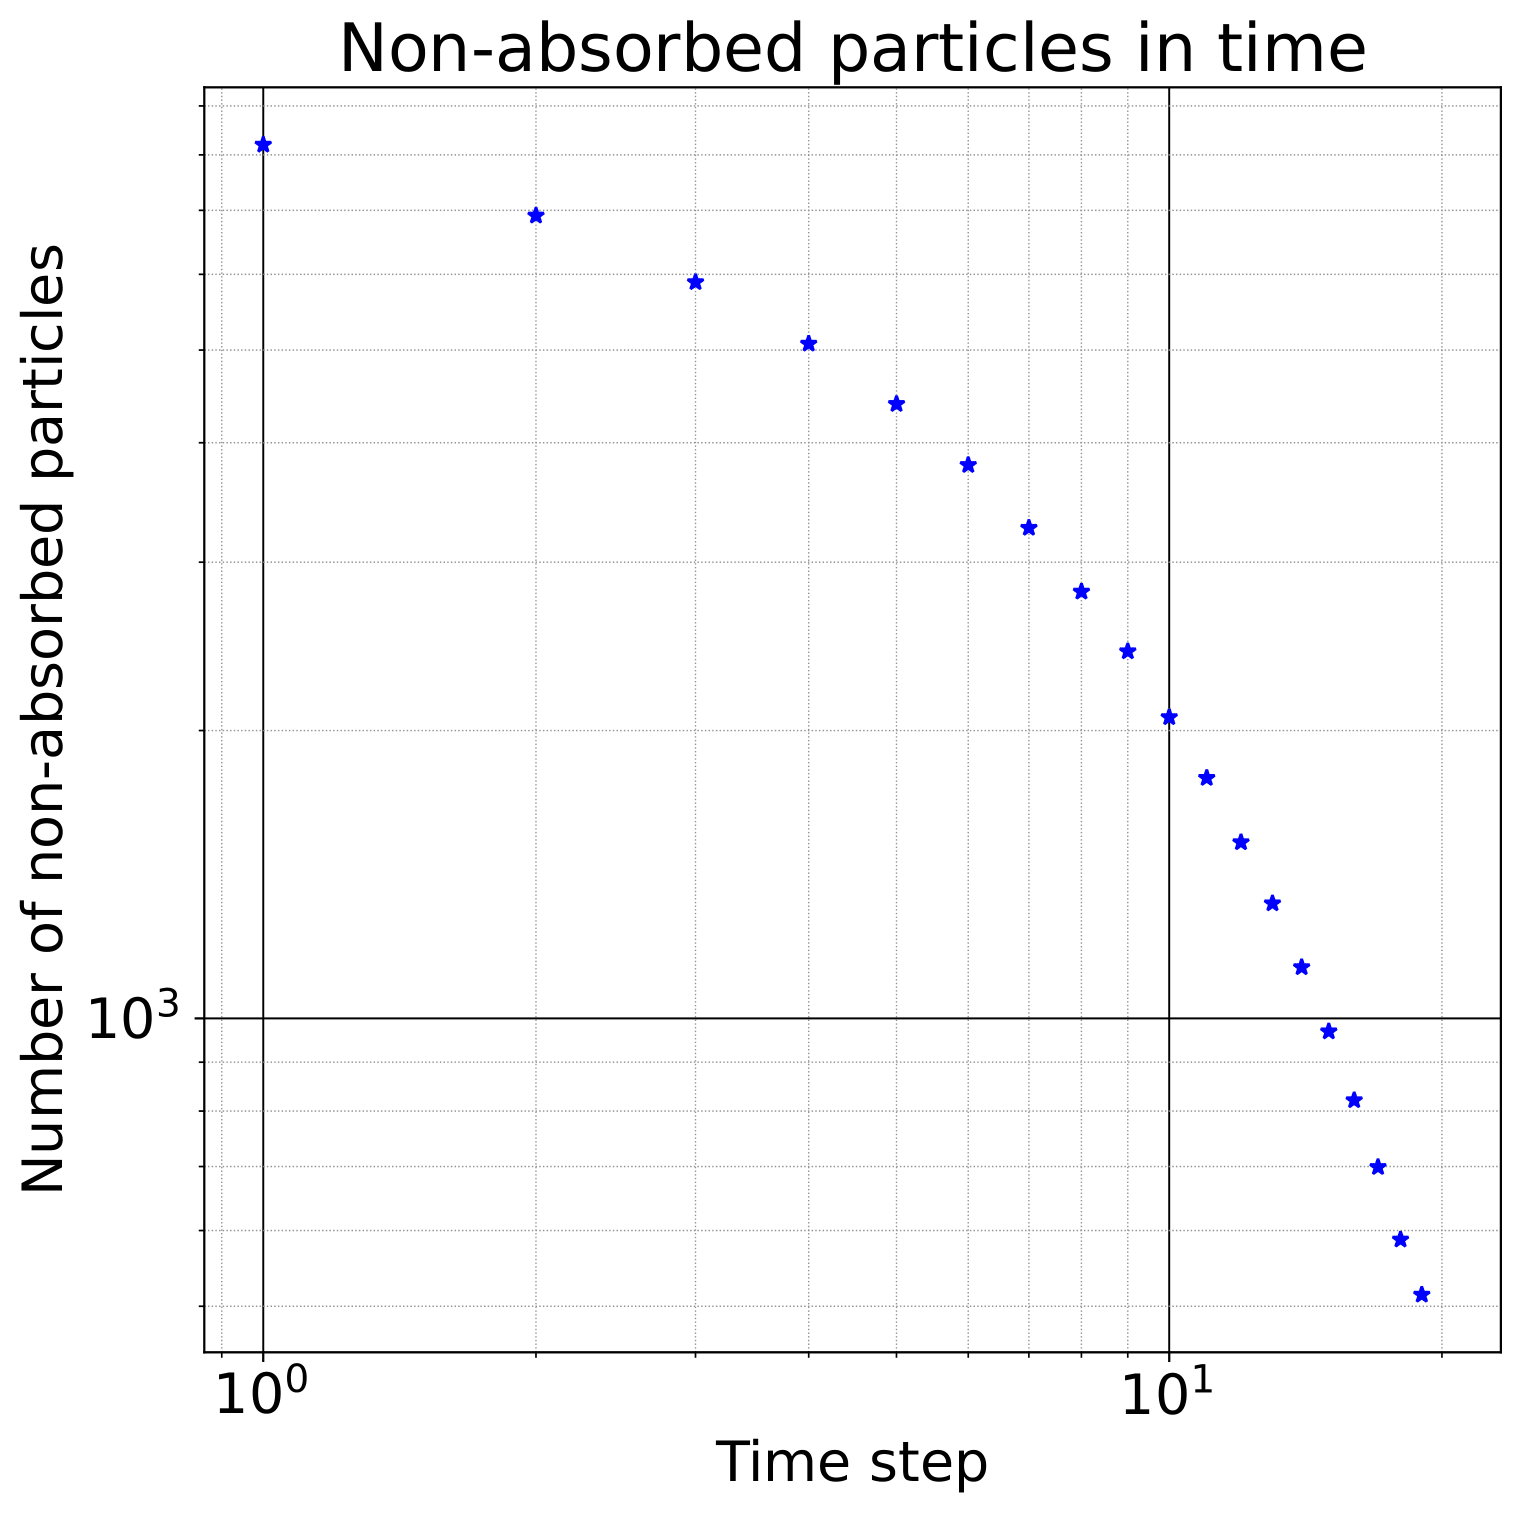
\includegraphics[width=\textwidth]{images/nonAbsParticles.png}
        \caption{Non-absorbed particles in time}
        \label{fig:subplotNonAbsPart}
    \end{subfigure}
    \hfill
    \begin{subfigure}[b]{0.45\textwidth}
        \centering
        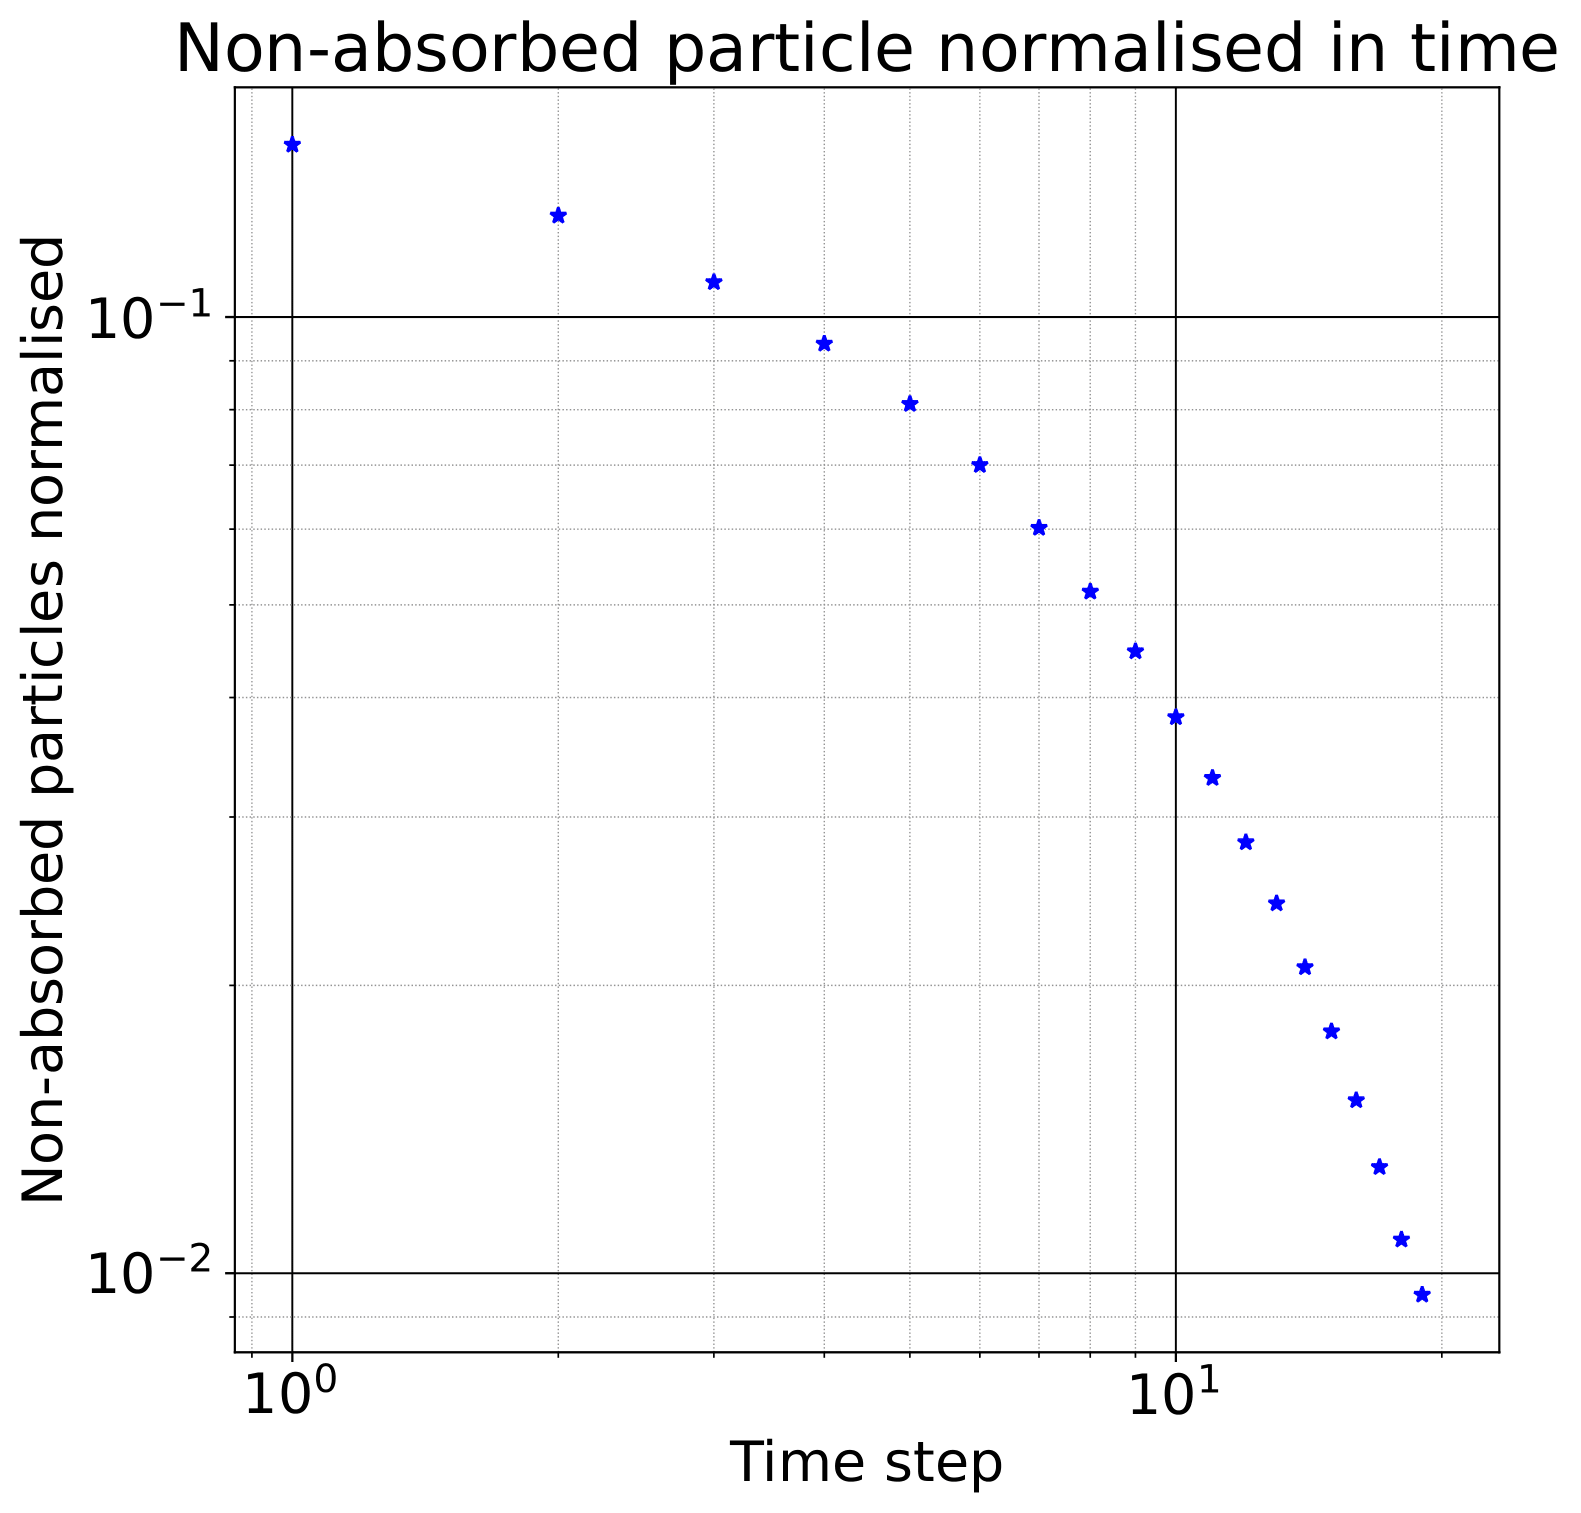
\includegraphics[width=\textwidth]{images/nonAbsParticlesNorm.png}
        \caption{Normalised number of non-absorbed particles in time}
        \label{fig:subplotNonAbsPartNorm}
    \end{subfigure}
    \caption{Non-absorbed particles in time normalised with initial total number of particles}
    \label{fig:AbsorptionInTime}
\end{figure}

\FloatBarrier  % Prevents figures from floating past this point
\subsection{Adsorbing boundaries: survival time distributions and effective reaction rates}
\subsubsection{Effect of diffusivity coefficient}
The following tables show the survival time distributions and effective reaction rates for particles' diffusion within a single fracture with reactive boundaries: as soon as the particles' trajectories cross the fracture's walls the particles get adsorbed (react) and disappear from the domain or, in other words, the adsorption probability is 100\%. The maximum number of time steps is 80000 and the time step is constant and equal to $dt=0.1$ which makes the overall maximum length of the simulation equal to 8000. Since the characteristic time is defined as $\tau_d=l^2/D_f$, where the fracture's aperture is $l=2$ the value of $\tau_D$ increases as the fracture's diffusion $D_f$ decreases. The number of particles for each simulation is $10^6$.
\begin{figure}[htbp]
    \centering
    \begin{subfigure}[b]{0.45\textwidth}
        \centering
        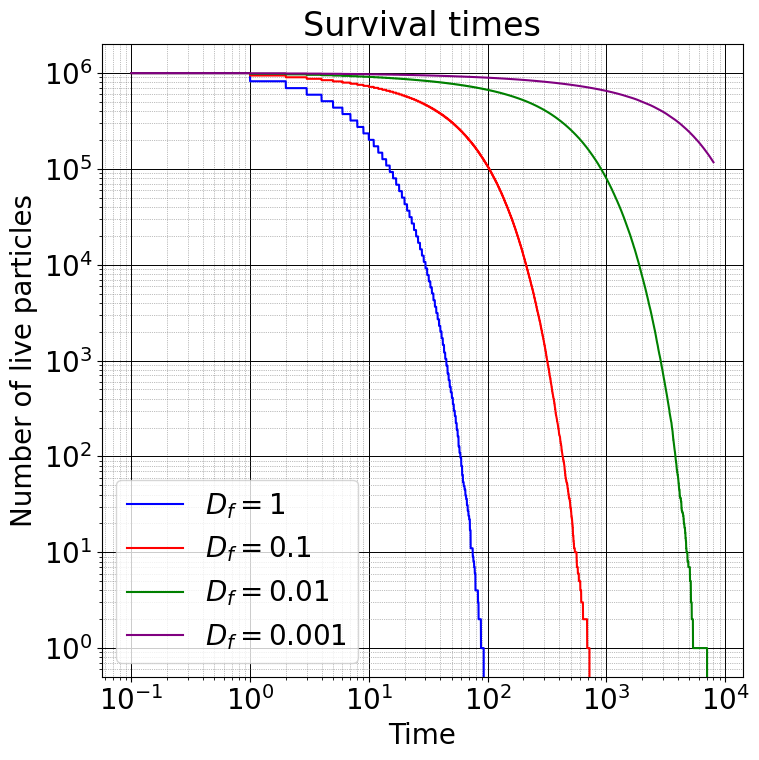
\includegraphics[width=\textwidth]{images/survTimeDistCompareDiff.png}
        \caption{Effect of diffusivity coefficient on survival time distribution for adsorbing boundary conditions}
    \end{subfigure}
    \hfill
    \begin{subfigure}[b]{0.45\textwidth}
        \centering
        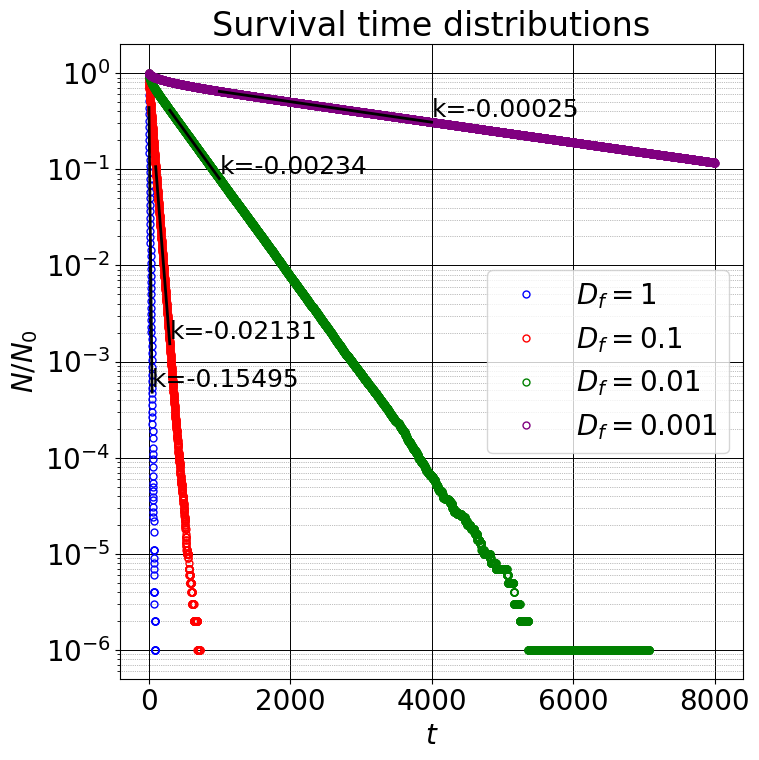
\includegraphics[width=\textwidth]{images/survTimeDistCompareDiffNorm.png}
        \caption{Effect of diffusivity coefficient on normalised survival time distribution for adsorbing boundary conditions}
    \end{subfigure}
    \caption{$10^6$ particles and 8000 time steps. The fracture's width is 2.}
    \label{fig:survTimeDiff}
\end{figure}

\begin{figure}[htbp]
    \centering
    \begin{subfigure}[b]{0.45\textwidth}
        \centering
        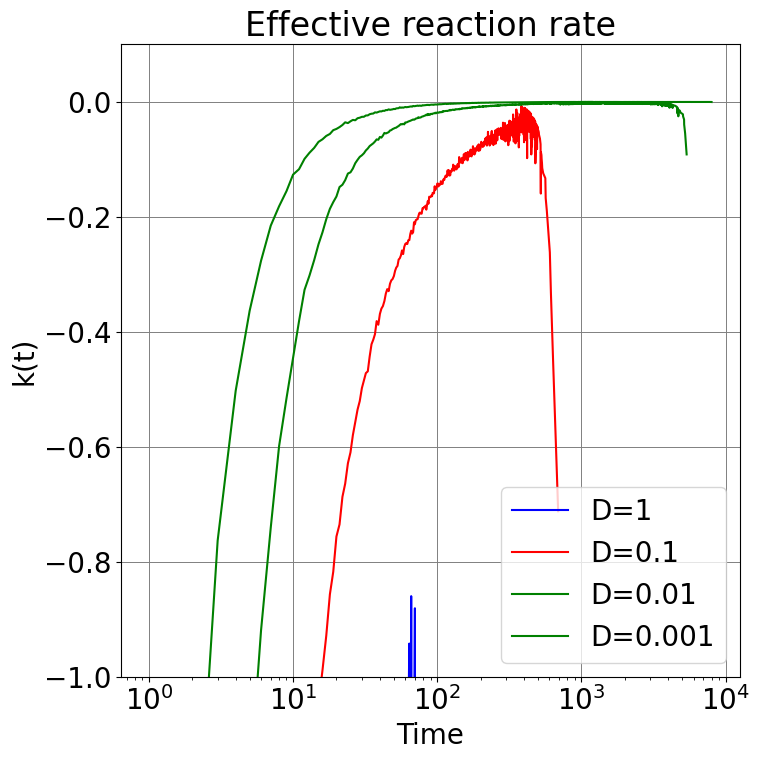
\includegraphics[width=\textwidth]{images/compareAdsRatesDiff.png}
        \caption{TO BE UPDATED}
    \end{subfigure}
    \hfill
    \begin{subfigure}[b]{0.45\textwidth}
        \centering
        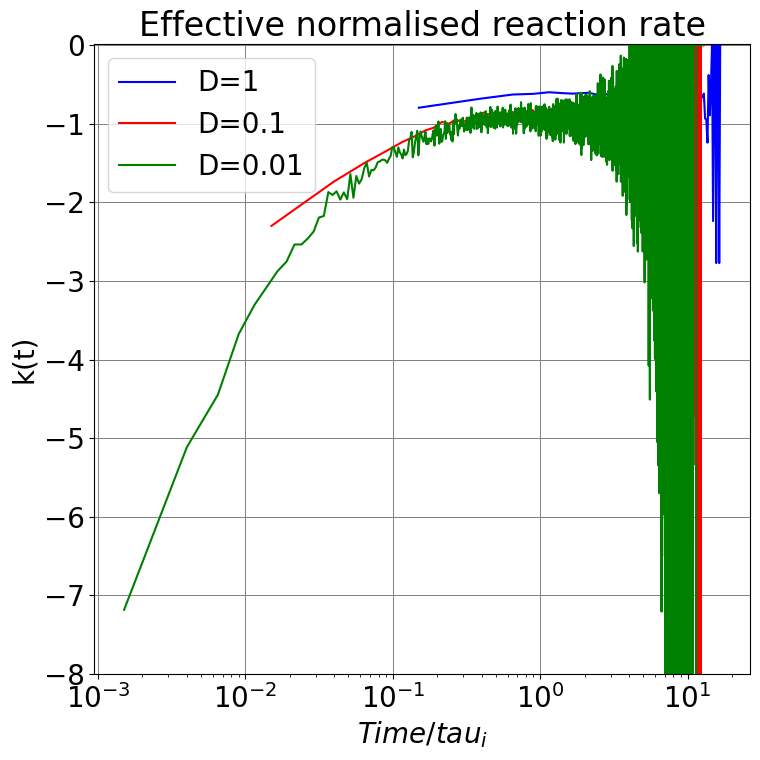
\includegraphics[width=\textwidth]{images/compareDiffNormAdsRates.png}
        \caption{Reaction rates for different diffusivity values from normalised surv time dist}
    \end{subfigure}
    \caption{Reaction rates for different diffusivity values}
    \label{fig:reactionRatesDiff}
\end{figure}

\FloatBarrier  % Prevents figures from floating past this point
\subsubsection{Effect of fracture's aperture}
\begin{figure}[htbp]
    \centering
    \begin{subfigure}[b]{0.45\textwidth}
        \centering
        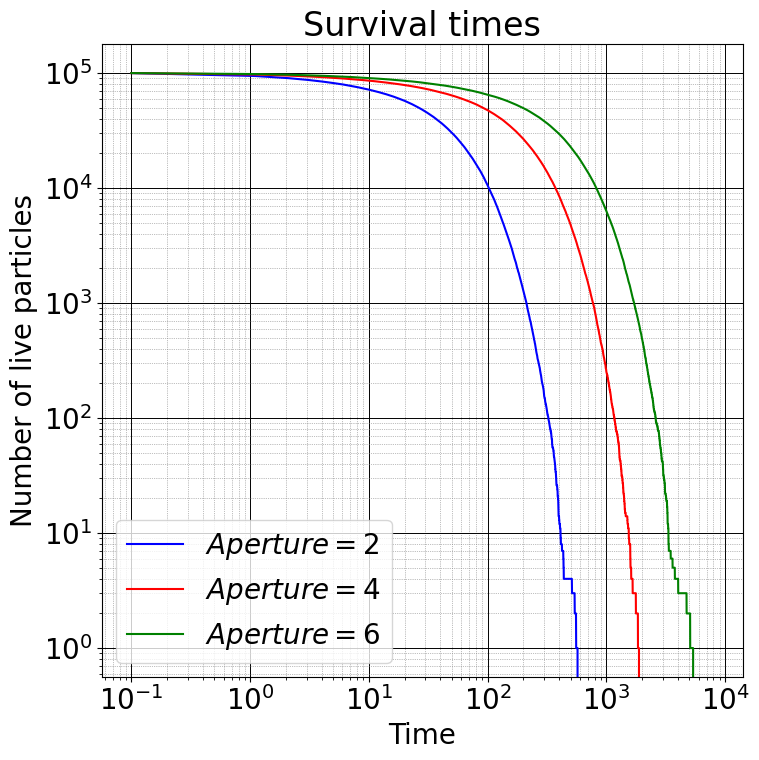
\includegraphics[width=\textwidth]{images/survTimeDistCompareApe.png}
        \caption{Effect of aperture's width on survival time distribution for adsorbing boundary conditions}
    \end{subfigure}
    \hfill
    \begin{subfigure}[b]{0.45\textwidth}
        \centering
        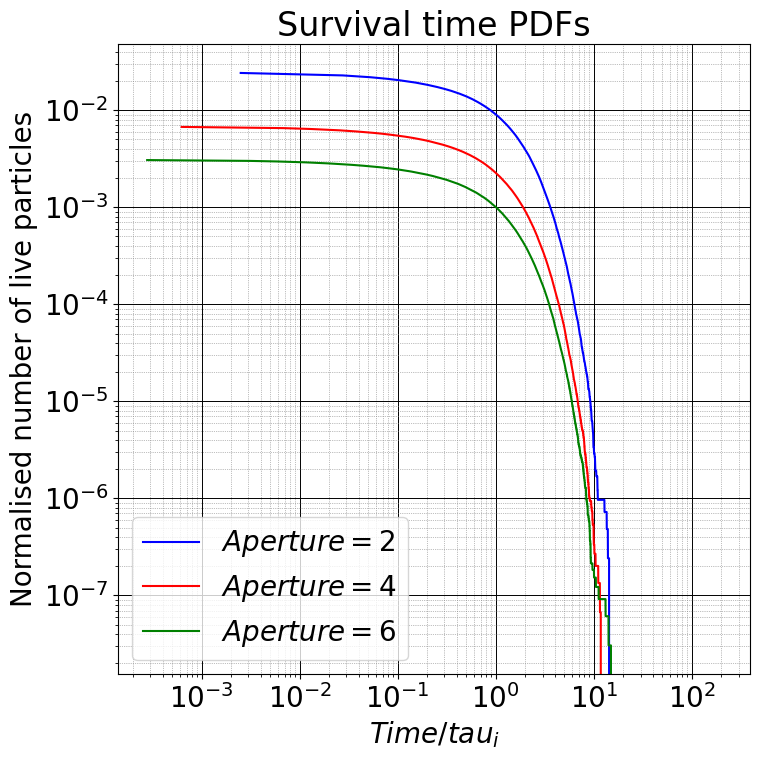
\includegraphics[width=\textwidth]{images/survTimeDistCompareApeNorm.png}
        \caption{Effect of aperture's width on normalised survival time distribution for adsorbing boundary conditions}
    \end{subfigure}
    \caption{$10^6$ particles and 8000 time steps. The diffusivity coefficient is 0.1.}
    \label{fig:survTimeape}
\end{figure}

\begin{figure}[htbp]
    \centering
    \begin{subfigure}[b]{0.45\textwidth}
        \centering
        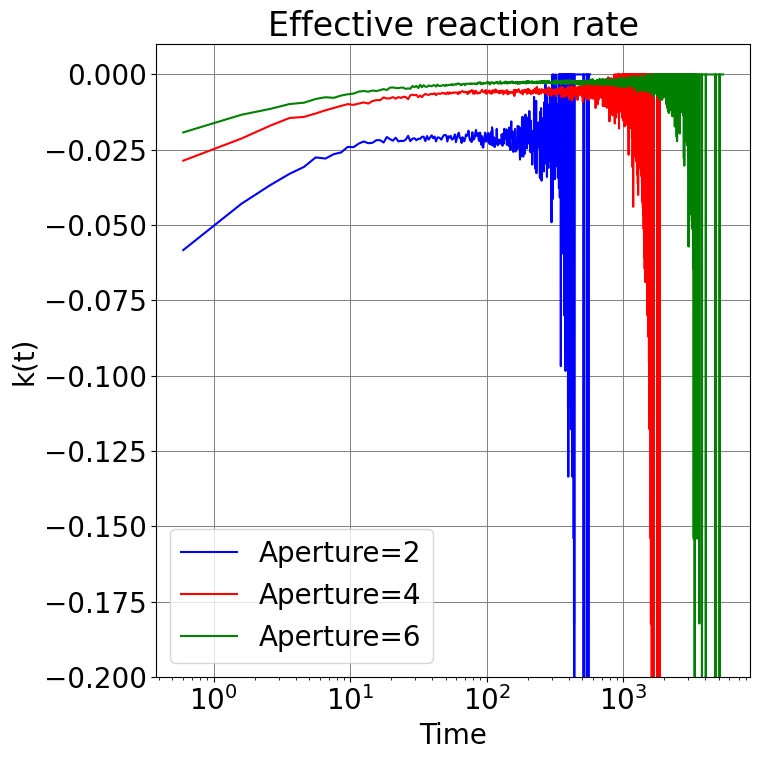
\includegraphics[width=\textwidth]{images/compareAdsRatesApe.png}
        \caption{Reaction rates for different values of apertures' width}
    \end{subfigure}
    \hfill
    \begin{subfigure}[b]{0.45\textwidth}
        \centering
        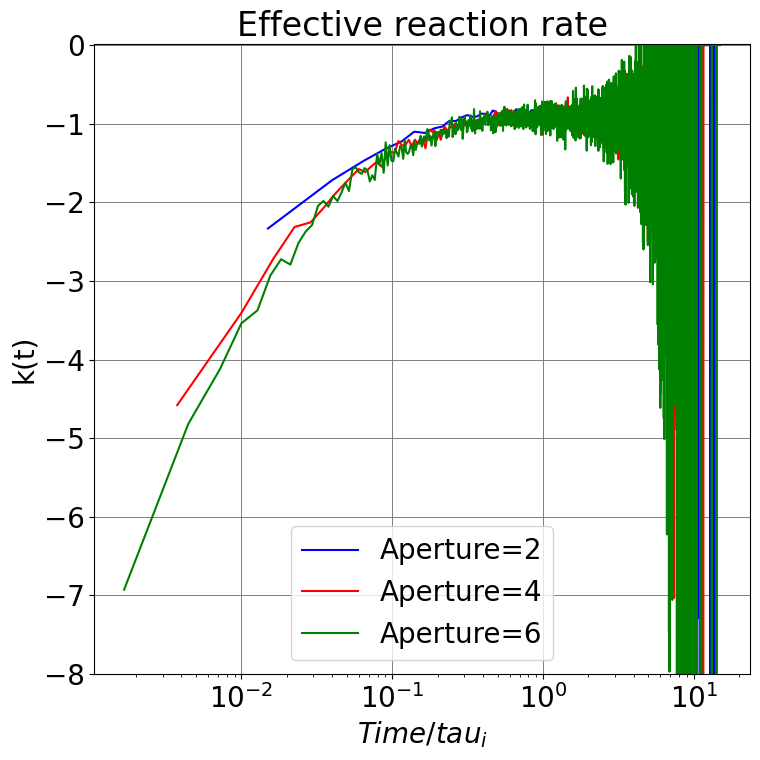
\includegraphics[width=\textwidth]{images/compareApeNormAdsRates.png}
        \caption{Reaction rates for different values of aperture's width from normalised survival time distributions}
    \end{subfigure}
    \caption{Reaction rates for different apertures' width}
    \label{fig:reactionRatesApe}
\end{figure}

\FloatBarrier  % Prevents figures from floating past this point
\subsubsection{Effect of adsorption probability}
\begin{figure}[htbp]
    \centering
    \begin{subfigure}[b]{0.45\textwidth}
        \centering
        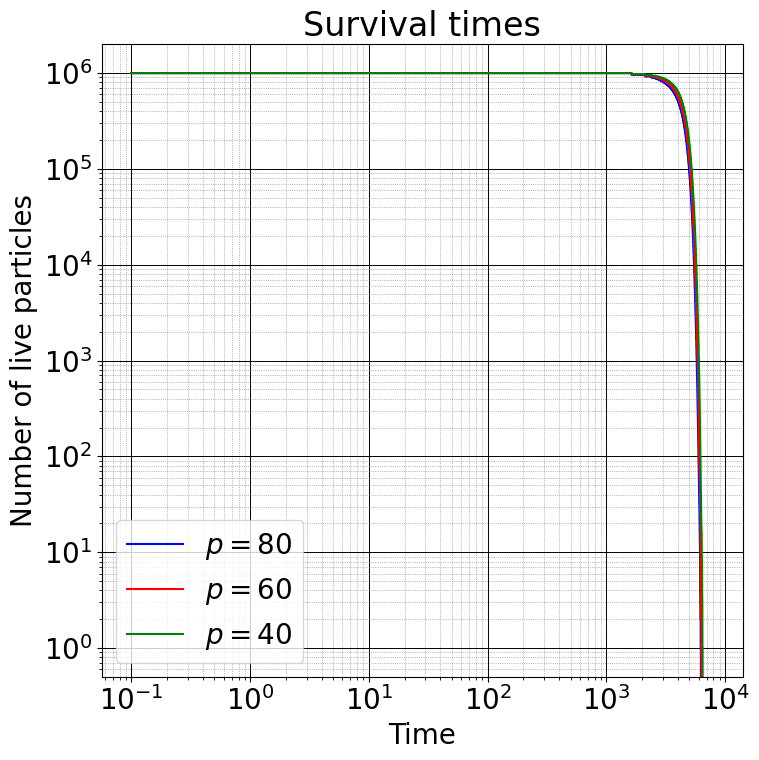
\includegraphics[width=\textwidth]{images/survTimeDistCompareProb.png}
        \caption{Effect of adsorption probability on survival time distribution for adsorbing boundary conditions}
    \end{subfigure}
    \hfill
    \begin{subfigure}[b]{0.45\textwidth}
        \centering
        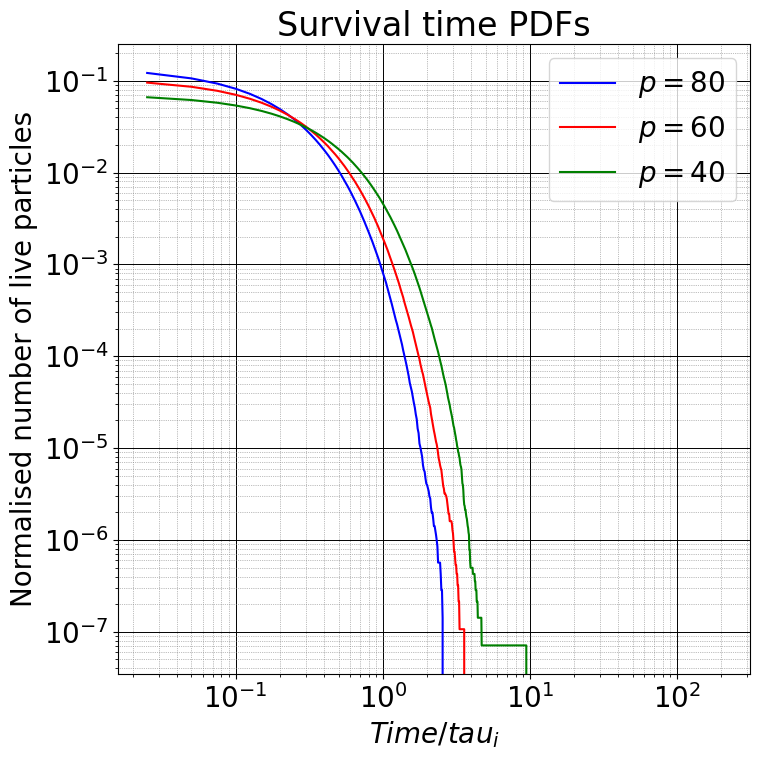
\includegraphics[width=\textwidth]{images/survTimeDistCompareProbNorm.png}
        \caption{Effect of adsorption probability on normalised survival time distribution for adsorbing boundary conditions}
    \end{subfigure}
    \caption{$10^6$ particles and 8000 time steps. The diffusivity coefficient is 0.1.}
    \label{fig:survTimeAdsProb}
\end{figure}

\begin{figure}[htbp]
    \centering
    \begin{subfigure}[b]{0.45\textwidth}
        \centering
        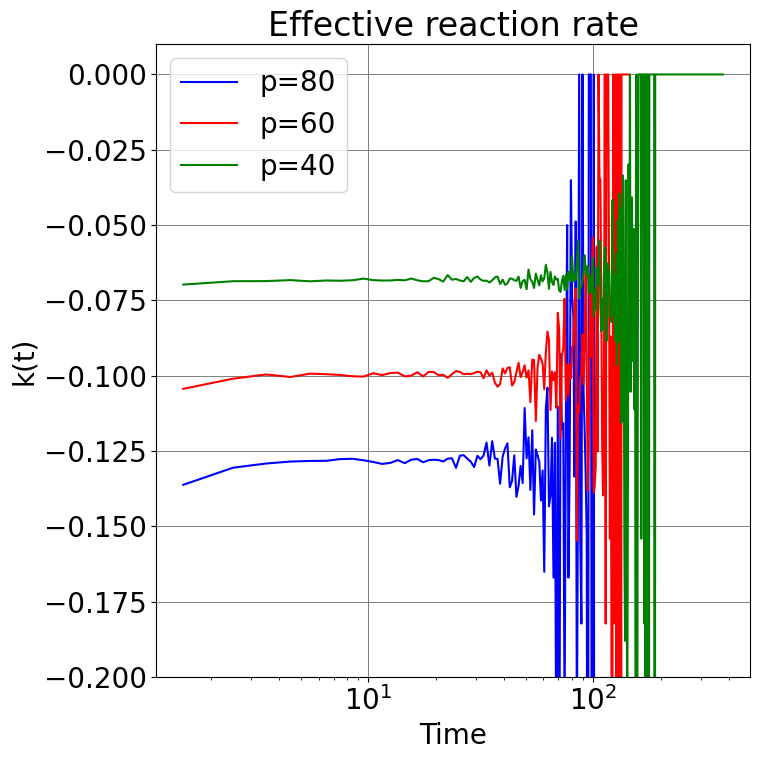
\includegraphics[width=\textwidth]{images/compareAdsRatesProb.png}
        \caption{Reaction rates for different values of adsorption probability}
    \end{subfigure}
    \hfill
    \begin{subfigure}[b]{0.45\textwidth}
        \centering
        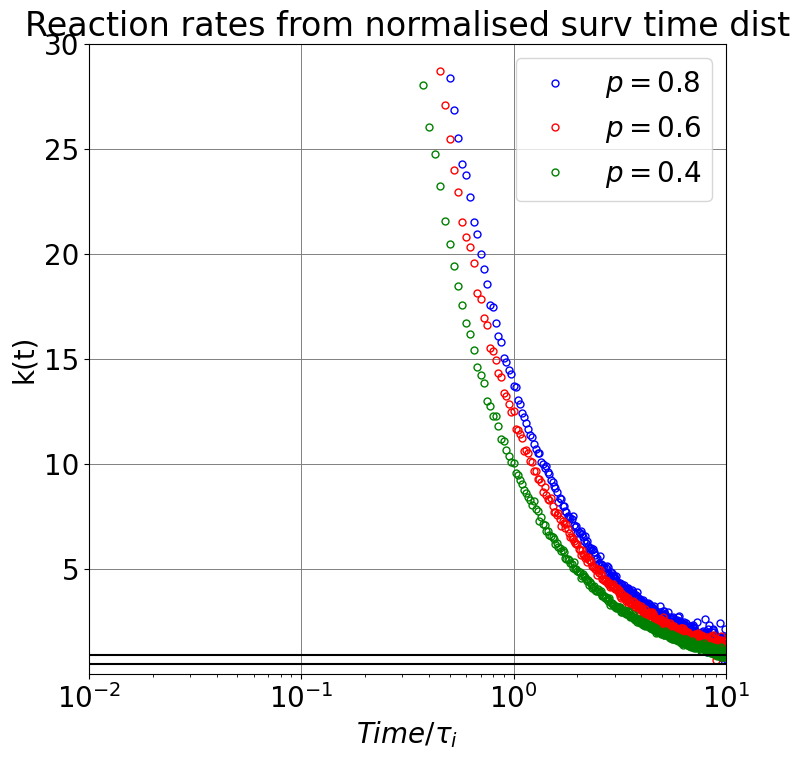
\includegraphics[width=\textwidth]{images/compareProbNormAdsRates.png}
        \caption{Reaction rates for different values of adsorption probability from normalised survival time distributions}
    \end{subfigure}
    \caption{Reaction rates for different adsorption probabilities}
    \label{fig:reactionRatesAdsProb}
\end{figure}

\FloatBarrier  % Prevents figures from floating past this point
\subsubsection{Effect of characteristic times}
\begin{figure}[htbp]
    \centering
    \begin{subfigure}[b]{0.48\textwidth}
        \centering
        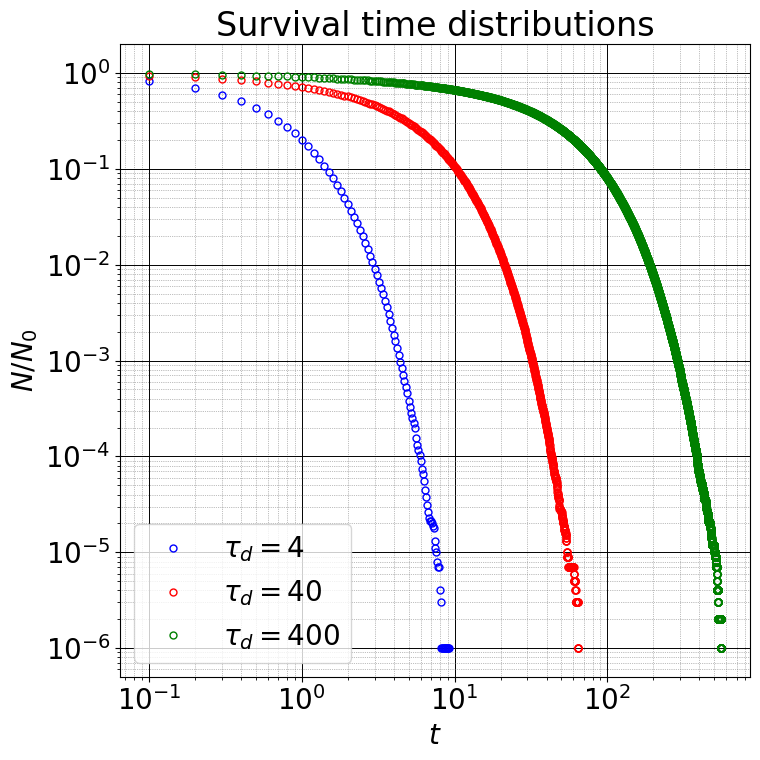
\includegraphics[width=\textwidth]{images/survTimeDistCompareTau.png}
        \caption{Effect of different characteristic times on survival time distribution curves}
    \end{subfigure}
    \hfill
    \begin{subfigure}[b]{0.48\textwidth}
        \centering
        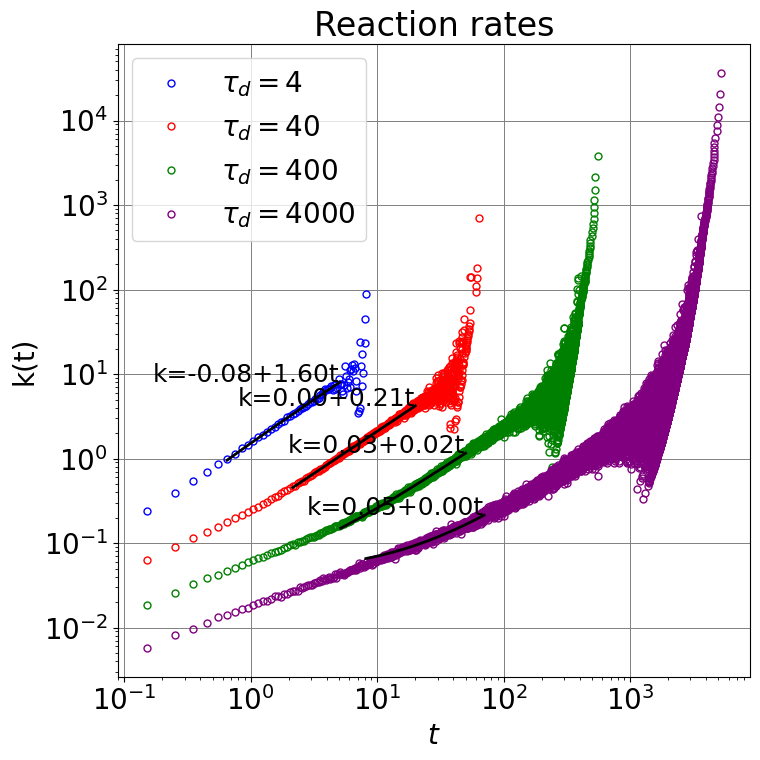
\includegraphics[width=\textwidth]{images/ratesCompareTau.png}
        \caption{Reaction rates for different characteristic times}
    \end{subfigure}
    \caption{$10^6$ particles and max 800 time steps with dt=0.1}
    \label{fig:survTimeDistTau}
\end{figure}

\begin{figure}[htbp]
    \centering
    \begin{subfigure}[b]{0.48\textwidth}
        \centering
        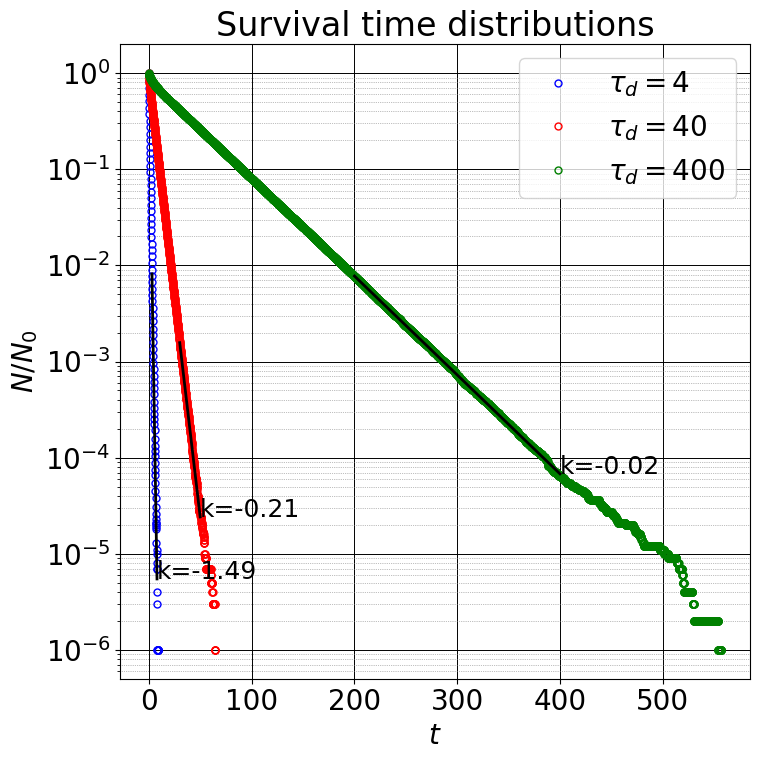
\includegraphics[width=\textwidth]{images/survTimeDistSemilogTau.png}
        \caption{Reaction rates for different characteristic times from the semilog tails}
    \end{subfigure}
    \hfill
    \begin{subfigure}[b]{0.48\textwidth}
        \centering
        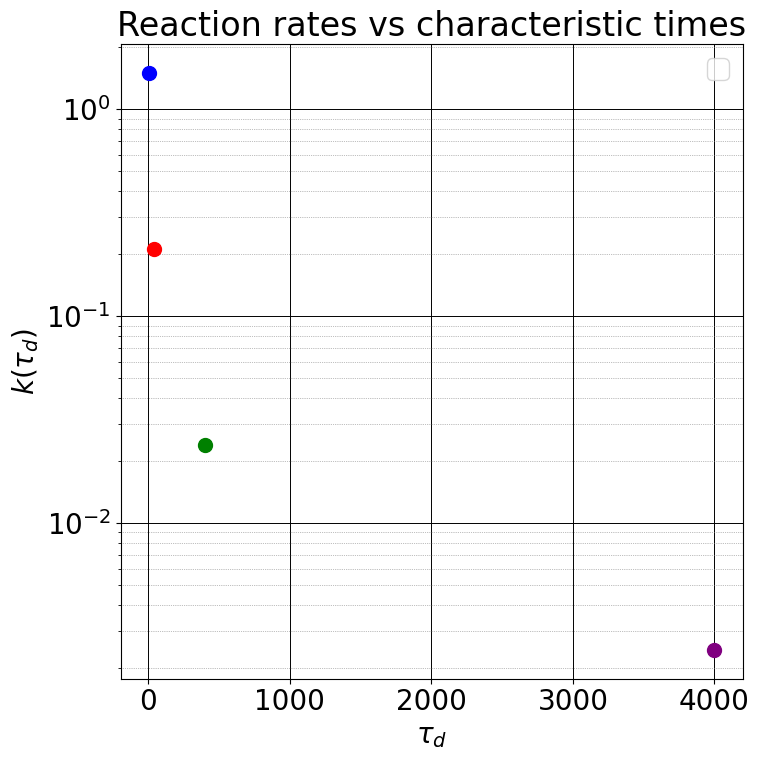
\includegraphics[width=\textwidth]{images/reactionVsTau.png}
        \caption{Reaction rates for different characteristic times}
    \end{subfigure}
    \caption{$10^6$ particles and max 800 time steps with dt=0.1}
    \label{fig:reactionRatesTau}
\end{figure}

\FloatBarrier  % Prevents figures from floating past this point
\subsubsection{Effect of adsorption probabilitiy}
\begin{figure}[htbp]
    \centering
    \begin{subfigure}[b]{0.48\textwidth}
        \centering
        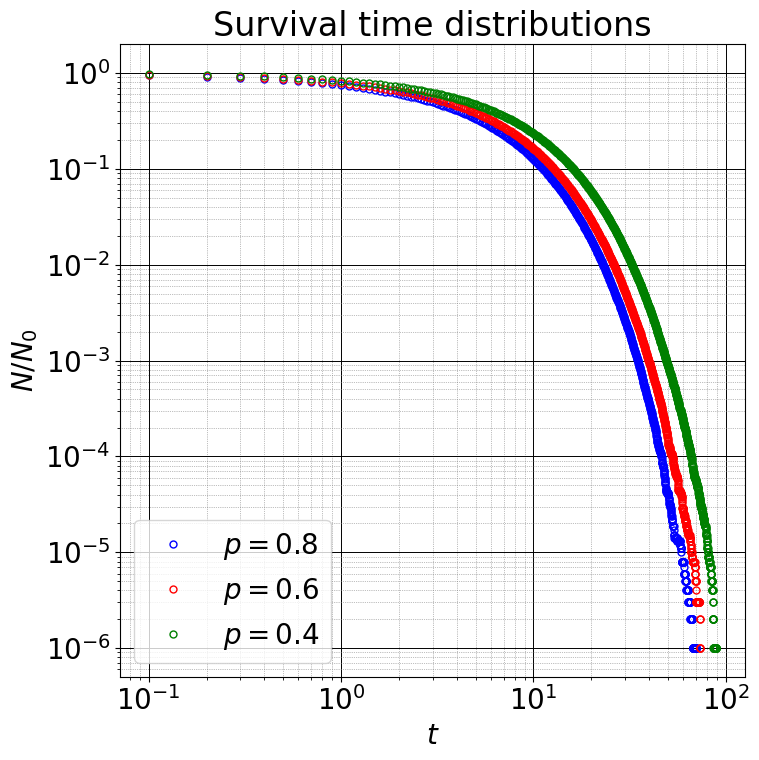
\includegraphics[width=\textwidth]{images/survTimeDistCompareAdsProb.png}
        \caption{Effect of different adsorption probabilities on survival time distribution curves}
    \end{subfigure}
    \hfill
    \begin{subfigure}[b]{0.48\textwidth}
        \centering
        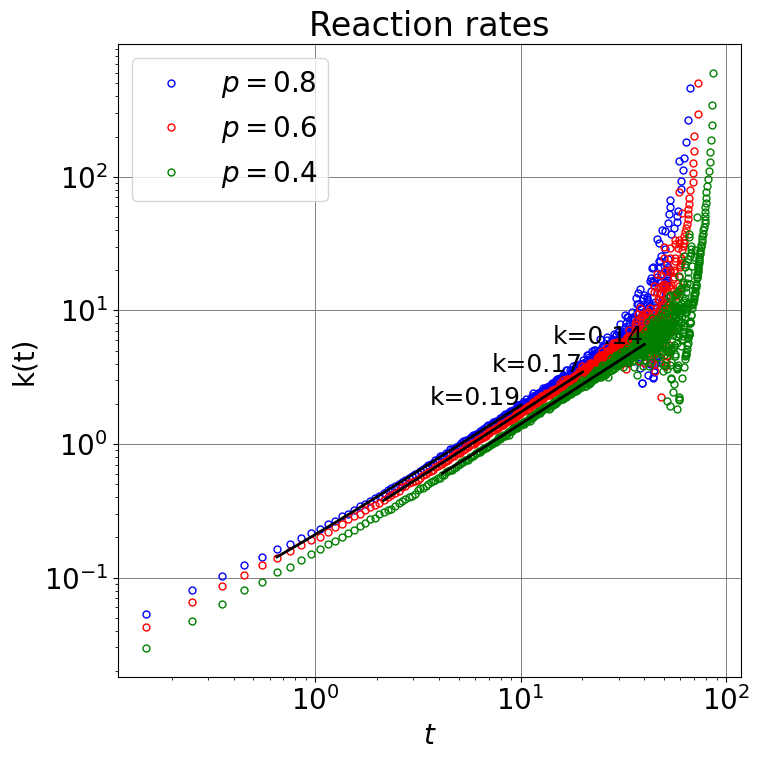
\includegraphics[width=\textwidth]{images/ratesCompareProb.png}
        \caption{Reaction rates for different adsorption probabilities}
    \end{subfigure}
    \caption{$10^6$ particles and max 800 time steps with dt=0.1}
    \label{fig:survTimeDistProb}
\end{figure}

\begin{figure}[htbp]
    \centering
    \begin{subfigure}[b]{0.48\textwidth}
        \centering
        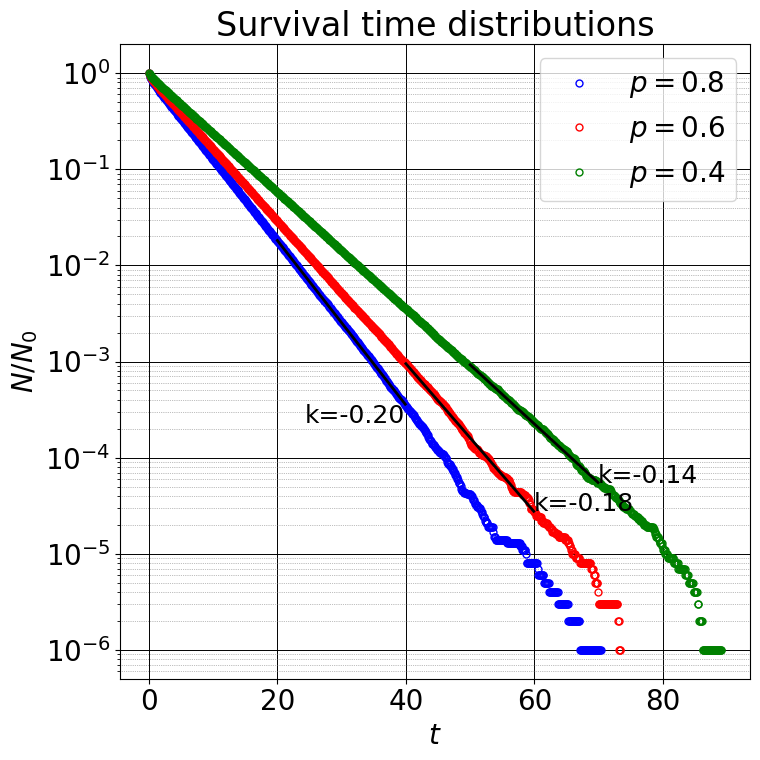
\includegraphics[width=\textwidth]{images/survTimeDistSemilogProb.png}
        \caption{Reaction rates for different characteristic times from the semilog tails}
    \end{subfigure}
    \hfill
    \begin{subfigure}[b]{0.48\textwidth}
        \centering
        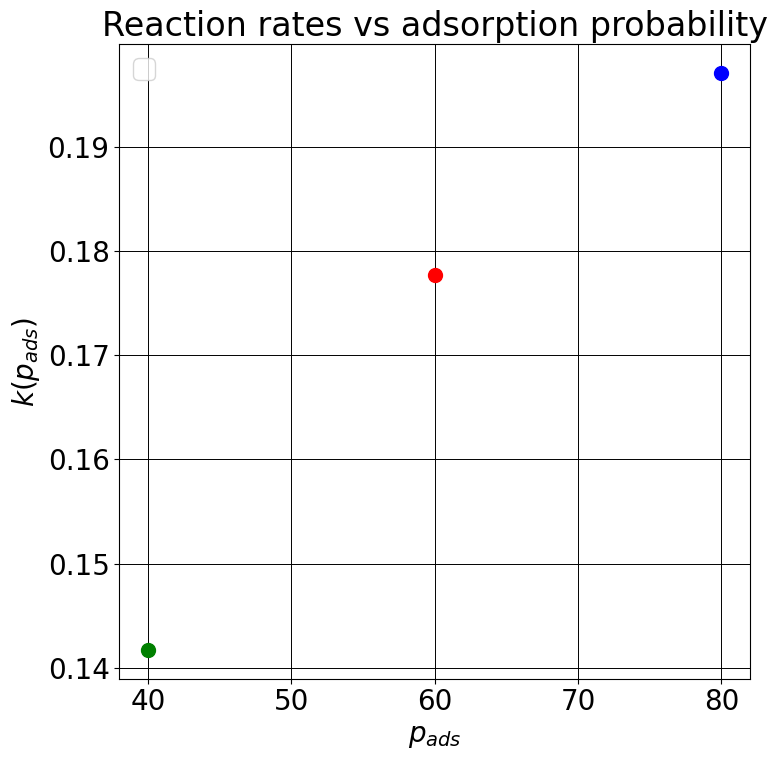
\includegraphics[width=\textwidth]{images/reactionVsProb.png}
        \caption{Reaction rates for different adsorption probabilities}
    \end{subfigure}
    \caption{$10^6$ particles and max 800 time steps with dt=0.1}
    \label{fig:reactionRatesProb}
\end{figure}

\FloatBarrier  % Prevents figures from floating past this point
\section{Well-mixed vs diffusion-limited}
\subsection{Survival time distribution and reaction rates}
\begin{figure}[htbp]
    \centering
    \begin{subfigure}[b]{0.45\textwidth}
        \centering
        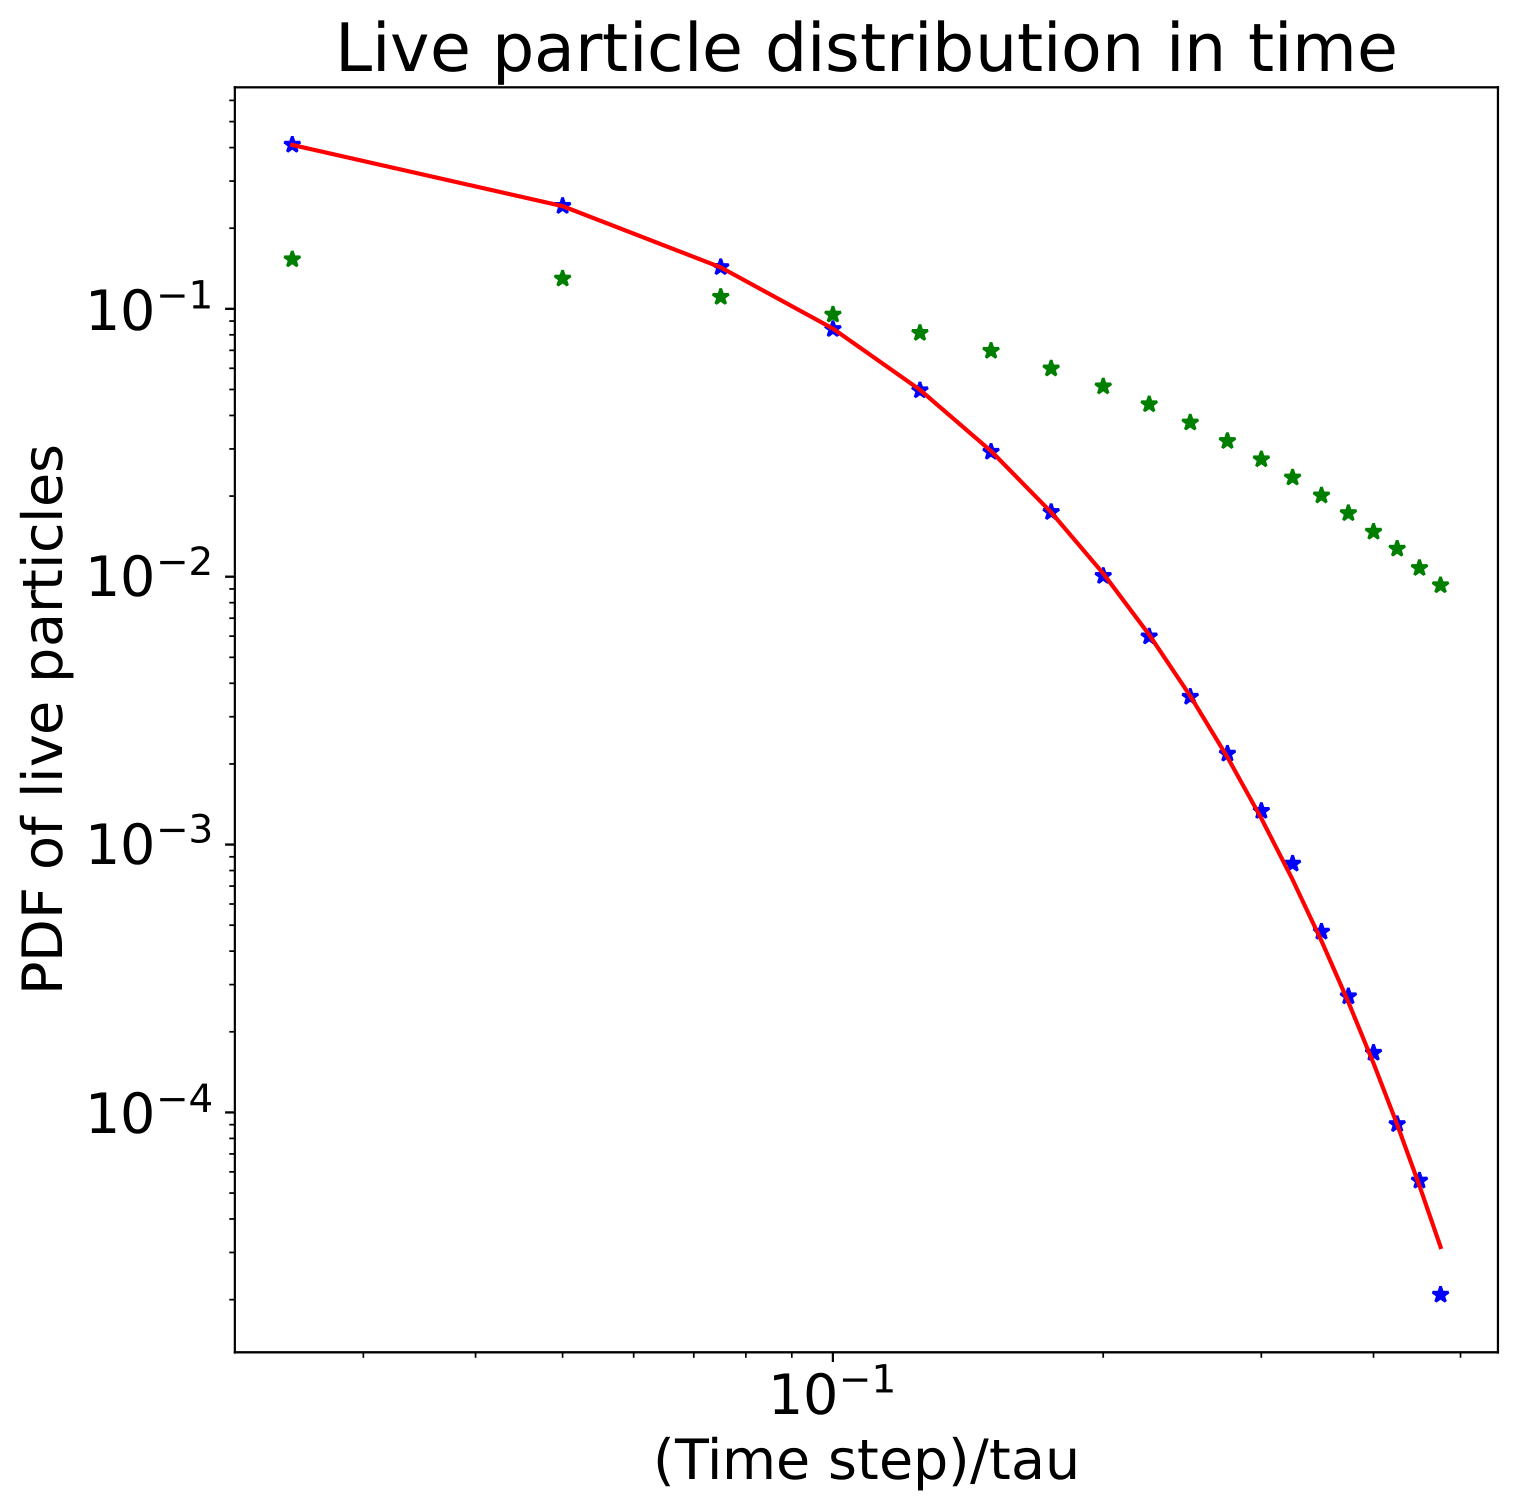
\includegraphics[width=\textwidth]{images/survTimeDistCompare.png}
        \caption{Survival time distribution curves from experimental well-mixed scenario and diffusion-limited experimental case.}
    \end{subfigure}
    \hfill
    \begin{subfigure}[b]{0.45\textwidth}
        \centering
        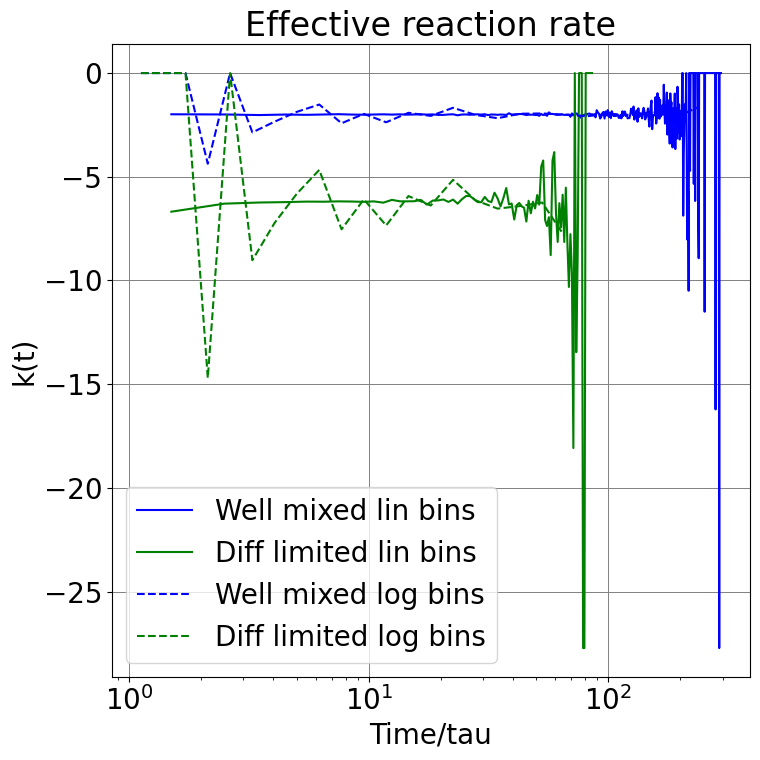
\includegraphics[width=\textwidth]{images/compareDecayDegradationRates.png}
        \caption{Reaction rates from experimental well-mixed scenario and diffusion-limited experimental case.}
    \end{subfigure}
    \caption{$10^6$ particles and 500 time steps. The value of the exponent k for the analytical case is 0.5.}
    \label{fig:survTimeAndRates}
\end{figure}

\begin{figure}[htbp]
    \centering
    \begin{subfigure}[b]{0.45\textwidth}
        \centering
        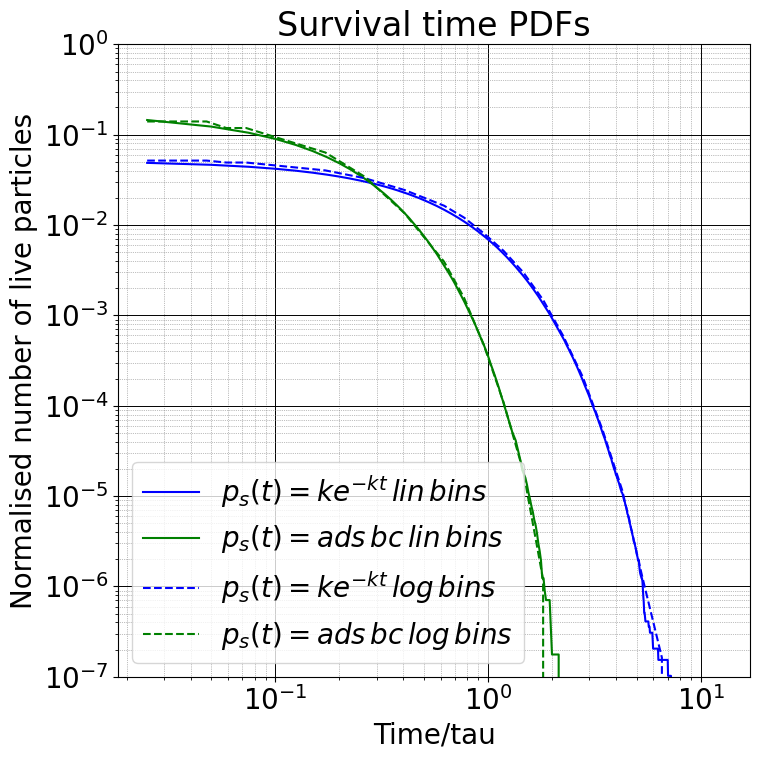
\includegraphics[width=\textwidth]{images/survTimeDistCompareNorm.png}
        \caption{Survival time distribution curves from experimental well-mixed scenario and diffusion-limited experimental case.}
    \end{subfigure}
    \hfill
    \begin{subfigure}[b]{0.45\textwidth}
        \centering
        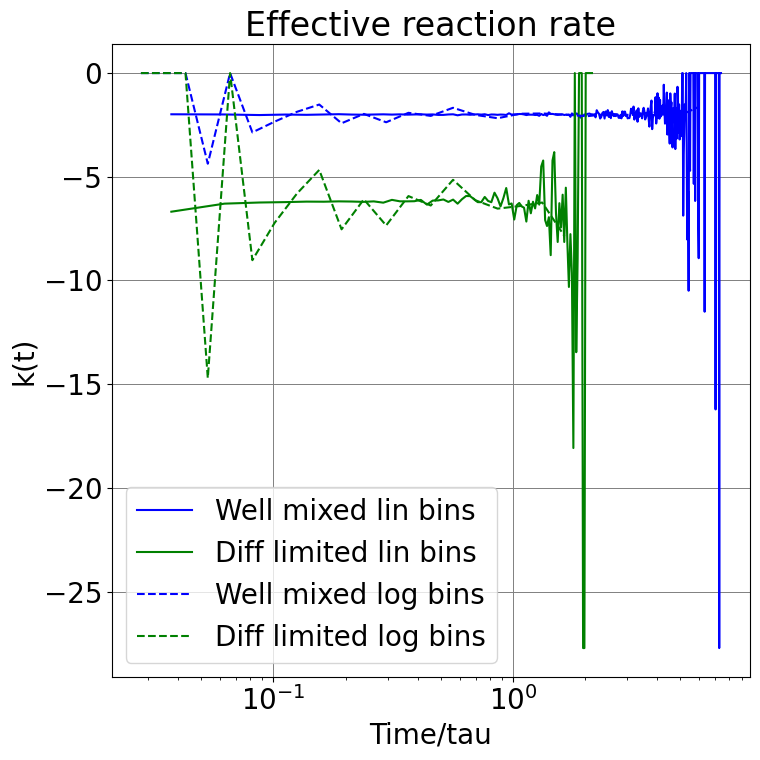
\includegraphics[width=\textwidth]{images/compareDecayDegradationRatesNorm.png}
        \caption{Reaction rates from experimental well-mixed scenario and diffusion-limited experimental case.}
    \end{subfigure}
    \caption{$10^6$ particles and 500 time steps. The value of the exponent k for the analytical case is 0.5.}
    \label{fig:survTimeAndRatesNorm}
\end{figure}

\FloatBarrier  % Prevents figures from floating past this point
\section{Matrix diffusion}
For each particle crossing from the fracture to the porous matrix, a random number from a uniform distribution over the interval 0 and 1 is drawn. If this number is higher than a threshold then the particle crosses the boundary otherwise it is elastically reflected. Following the approach of \cite{salamon2006review} we set the probability of a particle crossing the fracture-porous matrix boundary equal to:
\begin{equation}
    P_f = \frac{\sqrt{D_f}}{\sqrt{D_f}+\sqrt{D_m}}
    \label{eq:Salamon}
\end{equation}
\begin{figure}[htbp]
    \centering
    \begin{subfigure}[b]{0.45\textwidth}
        \centering
        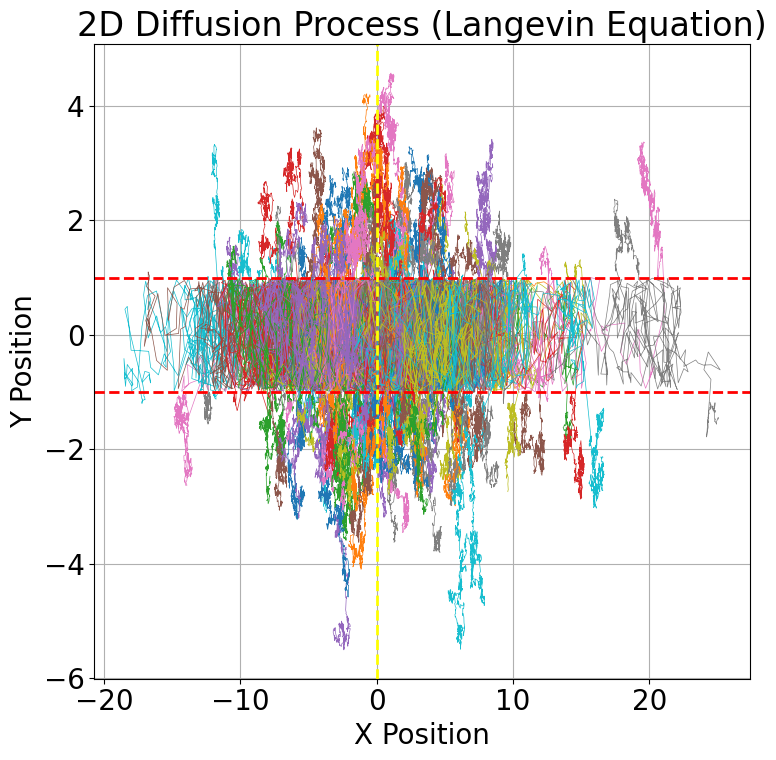
\includegraphics[width=\textwidth]{images/trajectoriesMatrixDiffusion.png}
        \caption{Trajectories from matrix diffusion implemented according to Semra 1993 and using Df=0.1 and Dm=0.001 and 100 particles and 1000 time steps}
        \label{fig:MatDiff}
    \end{subfigure}
    \hfill
    \begin{subfigure}[b]{0.45\textwidth}
        \centering
        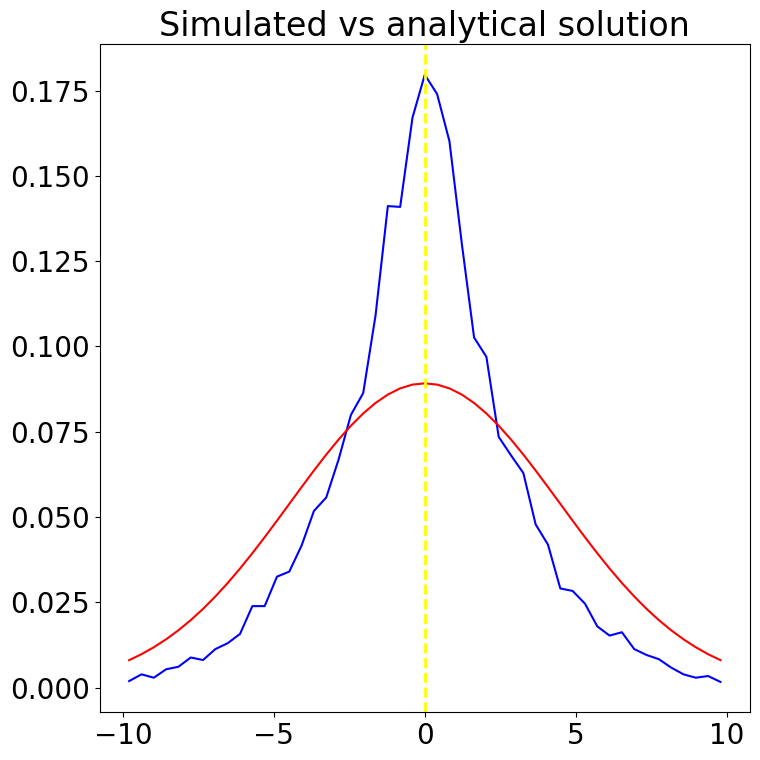
\includegraphics[width=\textwidth]{images/verificationMatrixDiffusion.png}
        \caption{Analytical solution vs numerical experiment using matrix diffusion and $10^4$ particles and $10^4$ time steps and recorded at t=100 time steps}
        \label{fig:MatrixDiffusionVerification}
    \end{subfigure}
    \caption{Verification against analytical solution for infinite domain}
    \label{fig:MatrixDiffusion}
\end{figure}
The table \ref{fig:MatrixDiffusionVerification} highlights the difference between the diffusion coefficient of the fracture and the one of the porous matrix: once a particle escapes from the fracture, its jumps are 100 times smaller compared to those that still live in the fracture. It follows that, the more impacts the more particles cross the border and the higher the concentration. Interesting enough, if the probability of matrix-to-fracture crossing is zero, after $10^4$ time steps no particles is left in the fracture, as shown in Figure \ref{fig:finalPosMatrixDiff}.
\begin{figure}[htbp]
    \centering
    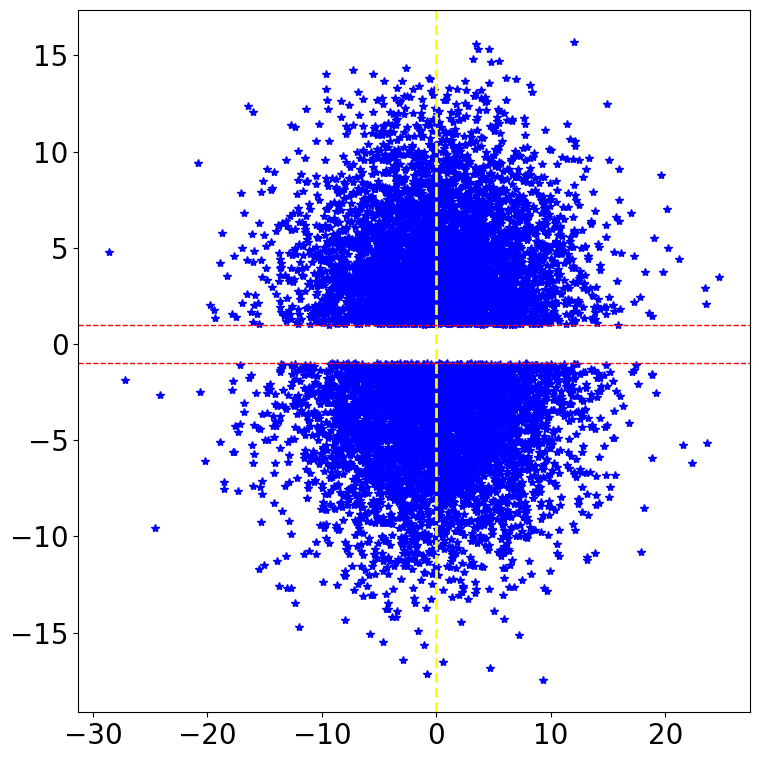
\includegraphics[width=0.5\textwidth]{images/finalPositionsMatrixDiffusion.png}
    \caption{Final position of $10^4$ particles after $10^4$ time steps}
    \label{fig:finalPosMatrixDiff}
\end{figure}

\FloatBarrier  % Prevents figures from floating past this point
\subsection{Verification: no probabilistic crossing between different diffusivity}
\begin{figure}[htbp]
    \centering
    \begin{subfigure}[b]{0.45\textwidth}
        \centering
        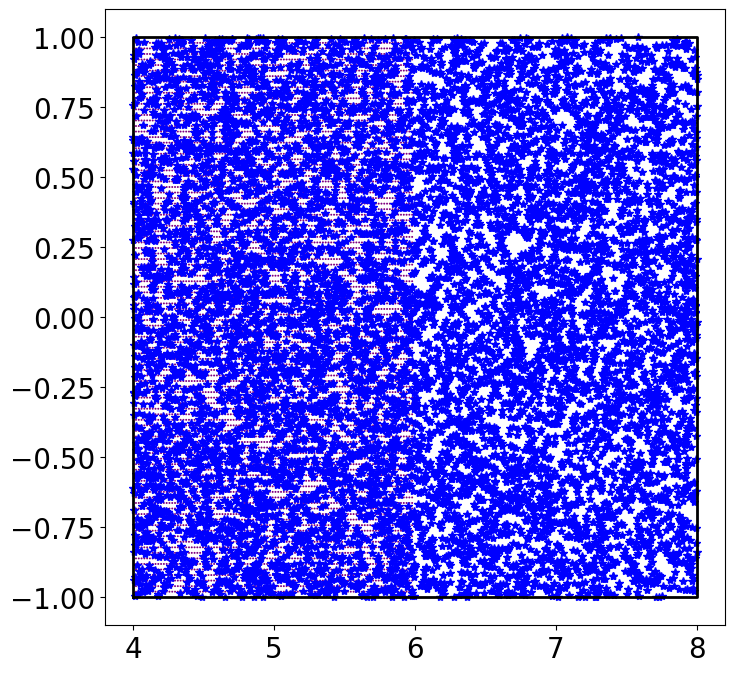
\includegraphics[width=\textwidth]{images/positionsDl01Dr01Rl0Rr0.png}
        \caption{No probability condition on crossing between the two diffusivity regions and Dl = Dr = 0.1}
    \end{subfigure}
    \hfill
    \begin{subfigure}[b]{0.45\textwidth}
        \centering
        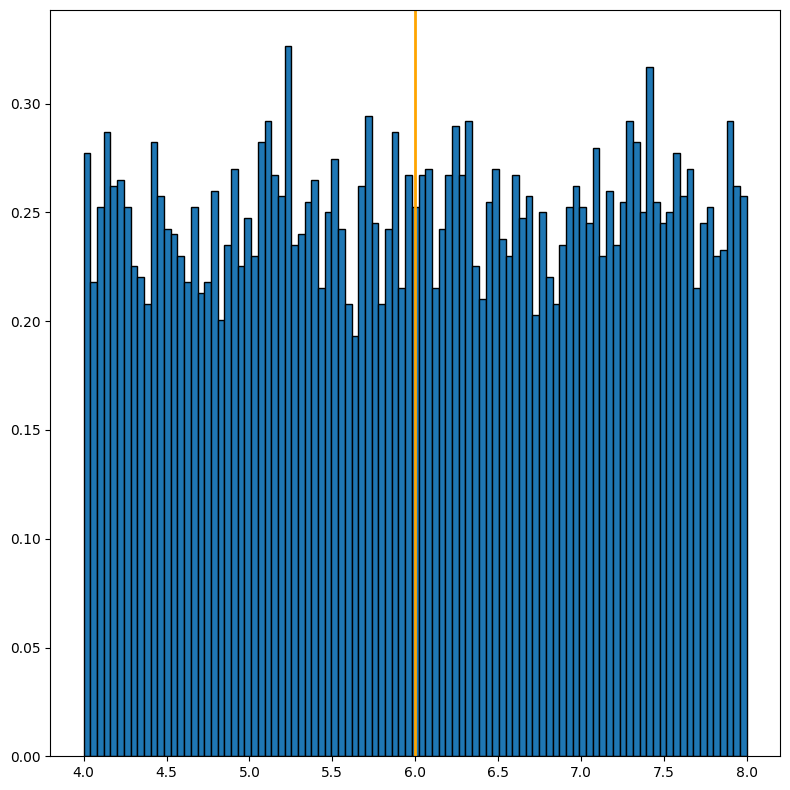
\includegraphics[width=\textwidth]{images/histDl01Dr01Rl0Rr0.png}
        \caption{Normalised histogram of particles' distribution along X at the end of the simulation}
    \end{subfigure}
    \caption{1e4 particles, 1e4 time steps, dt=1}
    \label{fig:MatrixDiffusion1}
\end{figure}

\begin{figure}[htbp]
    \centering
    \begin{subfigure}[b]{0.45\textwidth}
        \centering
        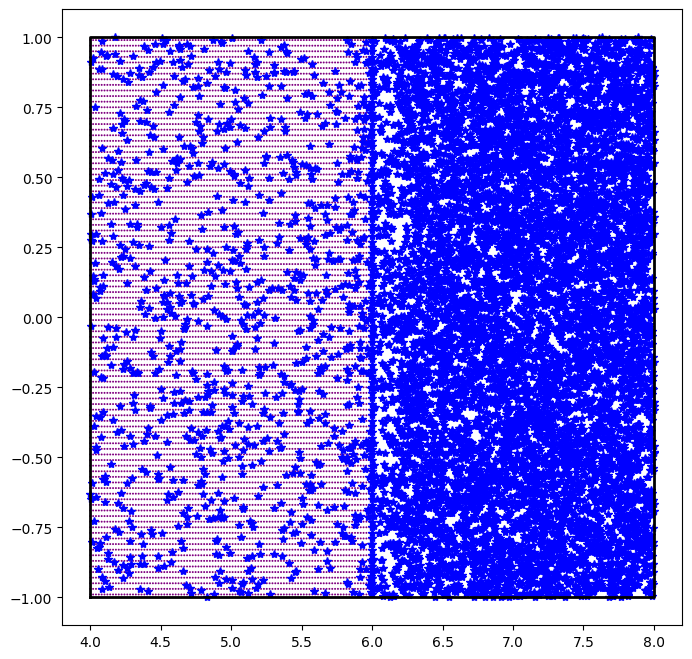
\includegraphics[width=\textwidth]{images/positionsDl01Dr001Rl0Rr0.png}
        \caption{No probability condition on crossing between the two diffusivity regions and Dl = 0.1 while Dr = 0.01}
    \end{subfigure}
    \hfill
    \begin{subfigure}[b]{0.45\textwidth}
        \centering
        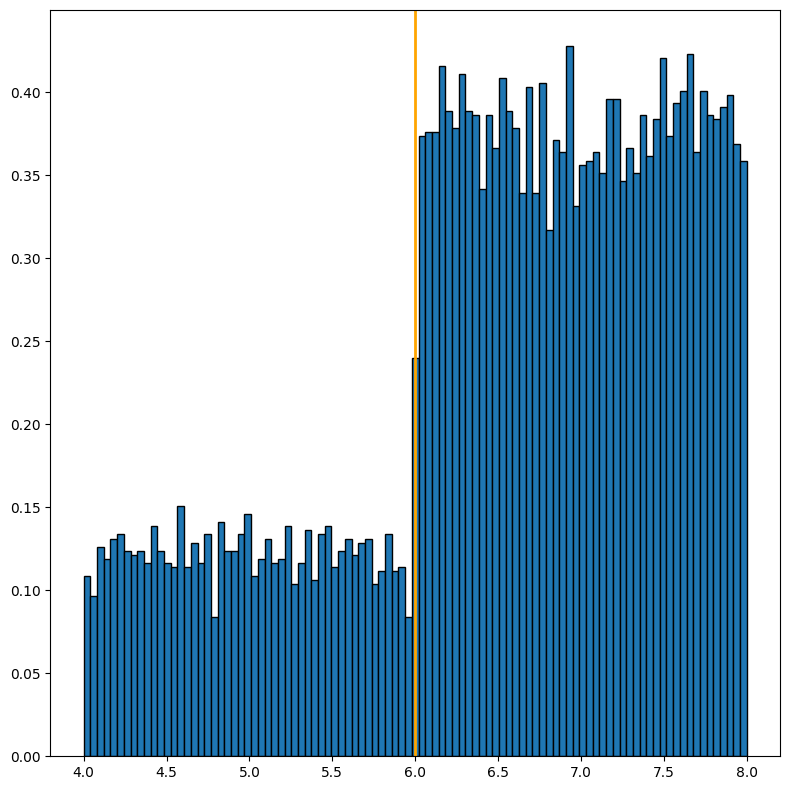
\includegraphics[width=\textwidth]{images/histDl01Dr001Rl0Rr0.png}
        \caption{Normalised histogram of particles' distribution along X at the end of the simulation}
    \end{subfigure}
    \caption{1e4 particles, 1e4 time steps, dt=1}
    \label{fig:MatrixDiffusion2}
\end{figure}

\FloatBarrier  % Prevents figures from floating past this point
\subsection{Verification: probabilistic boundary between different diffusivity}
\begin{figure}[htbp]
    \centering
    \begin{subfigure}[b]{0.45\textwidth}
        \centering
        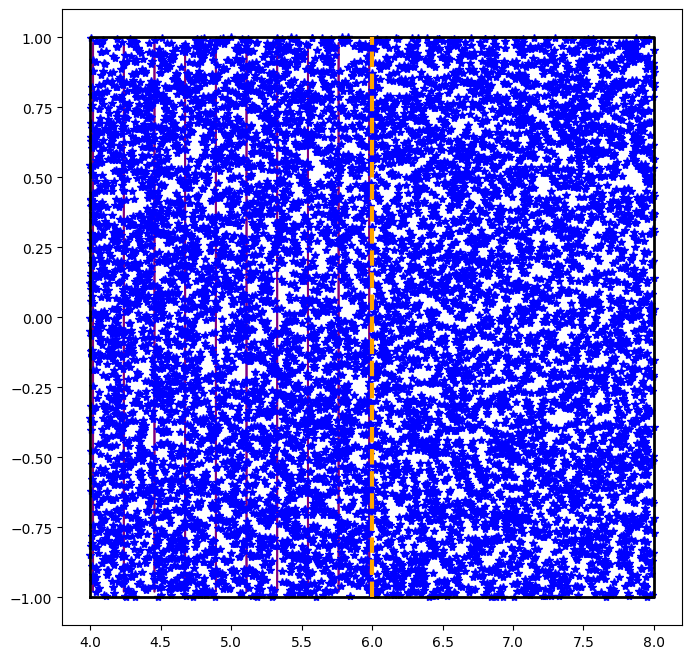
\includegraphics[width=\textwidth]{images/positionsDl01Dr01RlPlRrPr.png}
        \caption{Probability condition on crossing between the two diffusivity regions and Dl = Dr = 0.1}
    \end{subfigure}
    \hfill
    \begin{subfigure}[b]{0.45\textwidth}
        \centering
        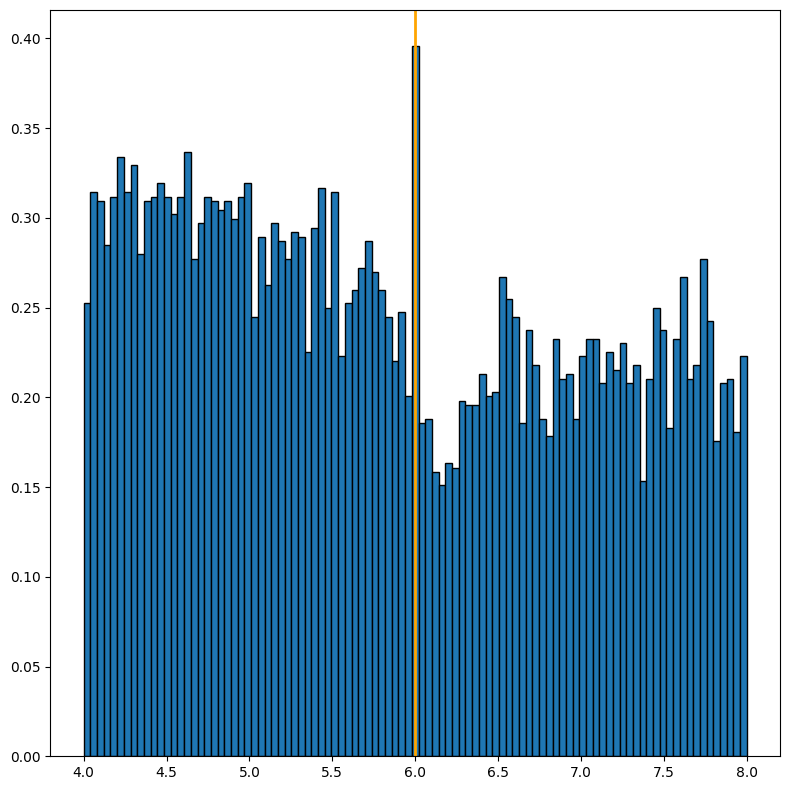
\includegraphics[width=\textwidth]{images/histDl01Dr01RlPlRrPr.png}
        \caption{Normalised histogram of particles' distribution along X at the end of the simulation}
    \end{subfigure}
    \caption{1e4 particles, 1e4 time steps, dt=1}
    \label{fig:MatrixDiffusion3}
\end{figure}

\begin{figure}[htbp]
    \centering
    \begin{subfigure}[b]{0.45\textwidth}
        \centering
        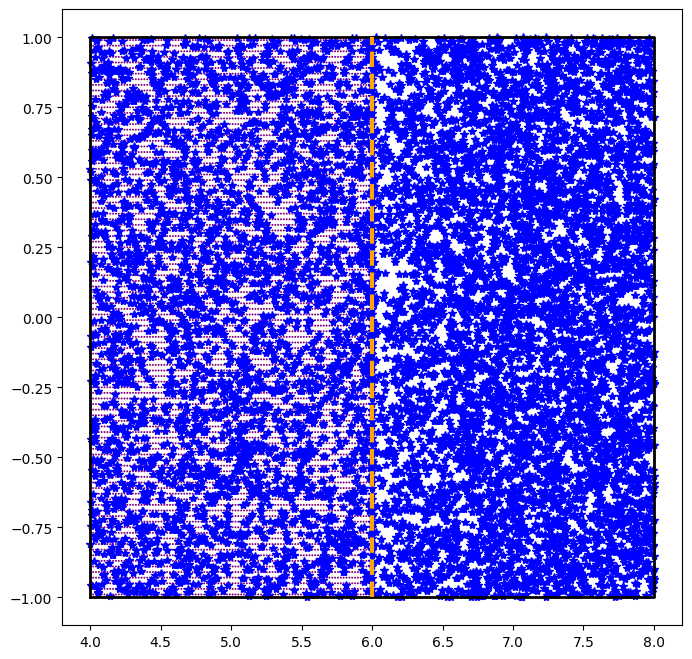
\includegraphics[width=\textwidth]{images/positionsDl01Dr001RlPlRrPr.png}
        \caption{Probability condition on crossing between the two diffusivity regions and Dl = 0.1 while Dr = 0.01}
    \end{subfigure}
    \hfill
    \begin{subfigure}[b]{0.45\textwidth}
        \centering
        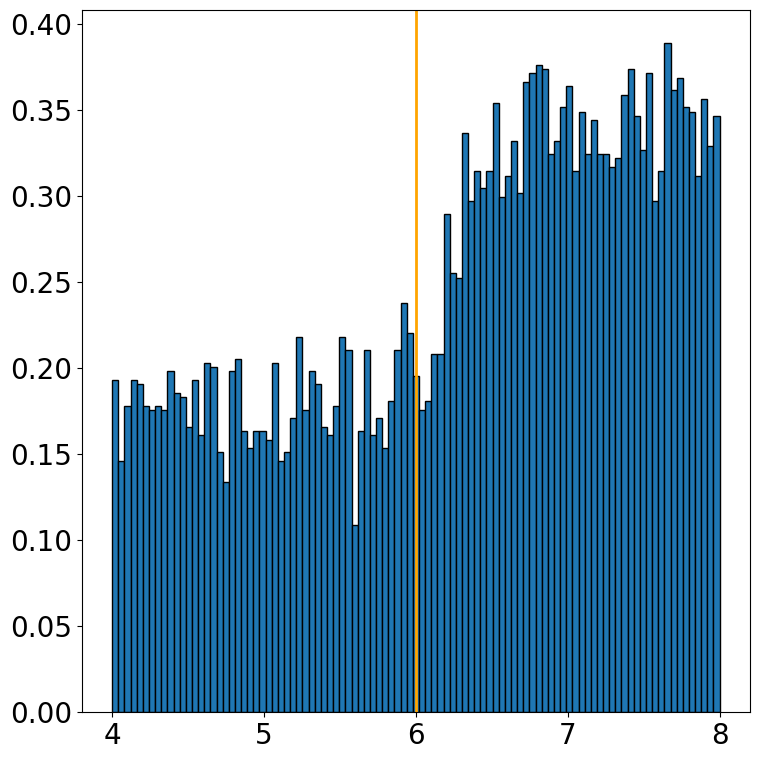
\includegraphics[width=\textwidth]{images/histDl01Dr001RlPlRrPr.png}
        \caption{Normalised histogram of particles' distribution along X at the end of the simulation}
    \end{subfigure}
    \caption{1e4 particles, 1e4 time steps, dt=1}
    \label{fig:MatrixDiffusion4}
\end{figure}

\FloatBarrier  % Prevents figures from floating past this point
\subsection{Radioactive decay in the porous matrix}
The aim of the following numerical experiments is to compare the degradation of particles under the effects of radioactive decay acting in different regions of the domain (fracture and porous matrix).
\begin{figure}[htbp]
    \centering
    \begin{subfigure}[b]{0.48\textwidth}
        \centering
        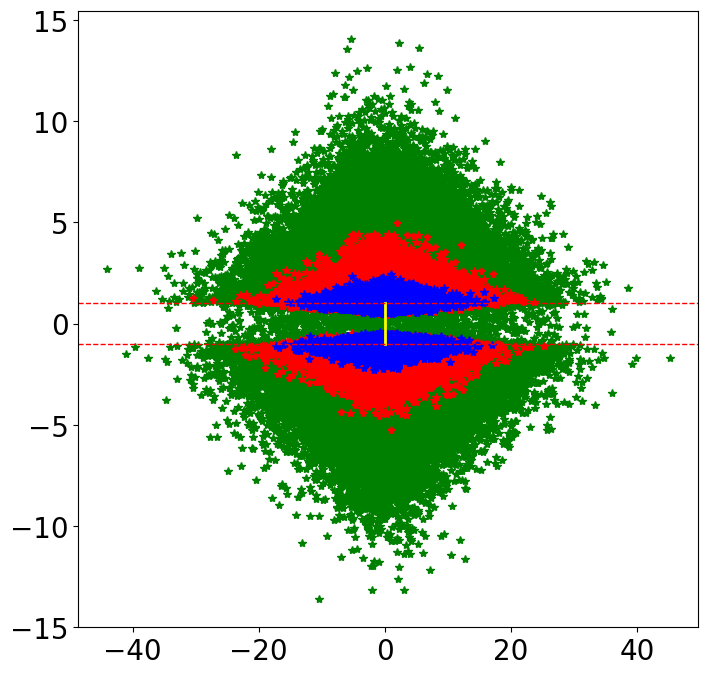
\includegraphics[width=\textwidth]{images/finalPositionMatrixDecay.png}
        \caption{Cloud of final positions for different radioactive decay in the porous matrix.}
    \end{subfigure}
    \hfill
    \begin{subfigure}[b]{0.48\textwidth}
        \centering
        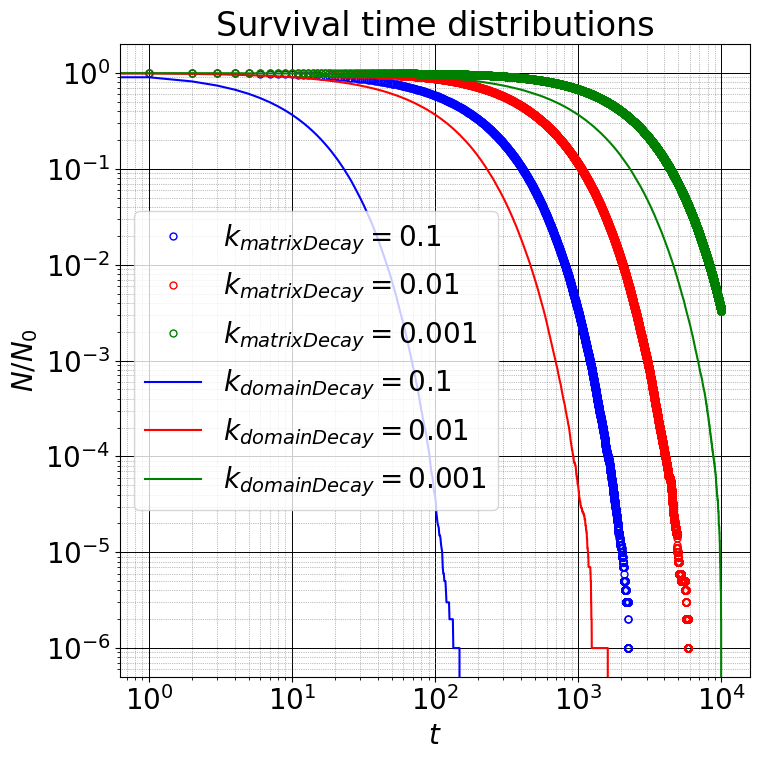
\includegraphics[width=\textwidth]{images/survTimeDistMatrixDecay.png}
        \caption{Survival time distributions for different radioactive decay in the porous matrix.}
    \end{subfigure}
    \caption{Different radioactive decay rates applied throughout the whole domain (fracture and porous matrix) vs decay rates for particles in porous matrix only. Setup: $10^6$ particles and max $10^6$ time steps with dt=1, Df=0.01 and Dm=0.001. The reflection probability is determined by Eq. \ref{eq:Salamon}.}
    \label{fig:survTimeDistMatrixDecay}
\end{figure}

\begin{figure}[htbp]
    \centering
    \begin{subfigure}[b]{0.48\textwidth}
        \centering
        \includegraphics[width=\textwidth]{images/ratesMatrixDecay.png}
        \caption{Reaction rates for different radioactive decays in the porous matrix.}
    \end{subfigure}
    \hfill
    \begin{subfigure}[b]{0.48\textwidth}
        \centering
        \includegraphics[width=\textwidth]{images/survTimeDistSemilogMatrixdecay.png}
        \caption{Reaction rates for different radioactive decays in the porous matrix.}
    \end{subfigure}
    \caption{$10^6$ particles and max $10^6$ time steps with dt=1, Df=0.01 and Dm=0.001.}
    \label{fig:reactionRatesMatrixDecay}
\end{figure}

\begin{figure}[htbp]
    \centering
    \begin{subfigure}[b]{0.48\textwidth}
        \centering
        \includegraphics[width=\textwidth]{images/survTimeDistLogBinsMatrixdecay.png}
        \caption{Survival time distribution from log-binning the values from figure \ref{fig:reactionRatesMatrixDecay} b.}
    \end{subfigure}
    \hfill
    \begin{subfigure}[b]{0.48\textwidth}
        \centering
        \includegraphics[width=\textwidth]{images/ratesMatrixDecayLog.png}
        \caption{Reaction rates for different radioactive decays in the porous matrix from the log-binning of the surv time distribution.}
    \end{subfigure}
    \caption{$10^6$ particles and max $10^6$ time steps with dt=1, Df=0.01 and Dm=0.001.}
    \label{fig:reactionRatesMatrixDecayLogBins}
\end{figure}

\begin{figure}[htbp]
    \centering
    \begin{subfigure}[b]{0.48\textwidth}
        \centering
        \includegraphics[width=\textwidth]{images/ratesMatrixDecaySpline.png}
        \caption{Reaction rates for different radioactive decays in the porous matrix from splines computed in figure \ref{fig:reactionRatesMatrixDecay} b.}
    \end{subfigure}
    \hfill
    \begin{subfigure}[b]{0.48\textwidth}
        \centering
        \includegraphics[width=\textwidth]{images/effVsDecayRates.png}
        \caption{Effective reaction rate vs radioactive decays in the porous matrix. The radioactive decay in the porous matrix ranges between 0.001 and 0.1.}
    \end{subfigure}
    \caption{$10^6$ particles and max $10^6$ time steps with dt=1, Df=0.01 and Dm=0.001.}
    \label{fig:effVsRadioactivedecays}
\end{figure}
Overall, the rates from figure \ref{fig:reactionRatesMatrixDecay} (a) and (b) compare well with those from figure \ref{fig:effVsRadioactivedecays} (a), which represent the derivatives of the cubic splines which fit the points in figure \ref{fig:reactionRatesMatrixDecay} (b). Last attempt for getting a smoother derivative is by binning the values from figure \ref{fig:reactionRatesMatrixDecay} (b) into log-spaced classes and compute the derivative of their average values.
\begin{figure}[htbp]
    \centering
    \includegraphics[width=0.5\textwidth]{images/effVsDecayRatesLogLog.png}
    \caption{Effective reaction rate vs radioactive decays in the porous matrix. The radioactive decay in the porous matrix ranges between 0.001 and 0.1. The results indicate a power law relation between the radioactive decay in the porous matrix and the corresponding values of effective decay rate. The effective decay rate can be approximated by $K_{eff} = e^{-3.87+0.51*log(K_{matrixDecay})}$.}
    \label{fig:KeffVsDmLog}
\end{figure}

\FloatBarrier  % Prevents figures from floating past this point
\subsection{Effect of molecular diffusion on radioactive decay}
As the molecular diffusion of particles in the porous matrix decreases, the effective decay rate decreases as well.
\begin{figure}[htbp]
    \centering
    \begin{subfigure}[b]{0.48\textwidth}
        \centering
        \includegraphics[width=\textwidth]{images/kEffVsDfDmRatio.png}
        \caption{Linear scale}
    \end{subfigure}
    \hfill
    \begin{subfigure}[b]{0.48\textwidth}
        \centering
        \includegraphics[width=\textwidth]{images/kEffVsDfDmRatioLogLog.png}
        \caption{Loglog scale}
    \end{subfigure}
    \caption{Effective radioactive decay for different values of molecular diffusion in the porous matrix. The characteristic time for all the simulation is $\tau_d=(u_b-l_b)^2/D_f=4/0.01=400$ while $D_m$ ranges between 0.01 and 0.00001. The value of the decay rate in the fracture is 0.01 and does not change between realisations. Setup: $10^6$ particles and max $10^6$ time steps with dt=1, Df=0.01 and Dm=0.001. The results indicate a power law relation between the ratio of matrix to fracture molecular diffusion and the corresponding values of effective decay rate. The effective decay rate can be approximated by $K_{eff} = e^{-5.32+0.38*log(D_m/D_f)}$.}
    \label{fig:KeffVsDm}
\end{figure}

\FloatBarrier  % Prevents figures from floating past this point
\section{OpenPNM}
Some tutorials adapted from: $https://openpnm.org/_examples/index.html$

\subsection{Network structures}
Some examples of pore-throat networks based on a cubic element.
\begin{figure}[htbp]
    \centering
    \begin{subfigure}[b]{0.48\textwidth}
        \centering
        \includegraphics[width=\textwidth]{images/3dStandardCubic.png}
        \caption{Standard 3x4x5 cubic network.}
    \end{subfigure}
    \hfill
    \begin{subfigure}[b]{0.48\textwidth}
        \centering
        \includegraphics[width=\textwidth]{images/3dConnectivity14.png}
        \caption{Cubic network where each node has 14 connections instead of 6.}
    \end{subfigure}
    \\
    \begin{subfigure}[b]{0.48\textwidth}
        \centering
        \includegraphics[width=\textwidth]{images/3dBcc.png}
        \caption{Body cubic centered network.}
    \end{subfigure}
    \hfill
    \begin{subfigure}[b]{0.48\textwidth}
        \centering
        \includegraphics[width=\textwidth]{images/3dFcc.png}
        \caption{Face centered cubic network.}
    \end{subfigure}
    \caption{Some examples of cubic networks.}
    \label{fig:CubicNetworks}
\end{figure}

\FloatBarrier  % Prevents figures from floating past this point
\subsection{Simulating Single Phase Transport}
Hagan-Poiseuille equation for fluid flow through a cylindrical tube:
\begin{equation}
    Q=\frac{\pi R^4}{8 \mu L} (P_{in}-P_{out})
\end{equation}
Conductance $g_h$:
\begin{equation}
    Q=g_h (P_{in}-P_{out})
\end{equation}
\begin{figure}[htbp]
    \centering
    \includegraphics[width=0.5\textwidth]{images/poiseuilleFlow.png}
    \caption{Hagen-Poiseuille flow verification using OpenPNM}
    \label{fig:poiseuille}
\end{figure}
Input data:
\begin{itemize}
    \item inlet pressure $P_{in} = 2 Pa = 2 kg/s^2m$;
    \item outlet flow rate $Q = 1 m^3/s$;
    \item conductance $g_h = 0.7035 m^4 s/kg$
\end{itemize}
Output:
\begin{itemize}
    \item outlet pressure $P_{out} = 0.578 Pa = 0.578 kg/s^2m$
\end{itemize}

\FloatBarrier  % Prevents figures from floating past this point
\subsection{3D cubic network with homogeneous pore and throat geometries}
Input data:
\begin{itemize}
    \item throat length: $1e-2$
    \item throat diameter: $1e-4$
    \item pore diameter: $1e-3$
    \item water viscosity: $0.00089$
    \item pressure left: $2$
    \item pressure right: $1$
\end{itemize}
\begin{figure}[htbp]
    \centering
    \includegraphics[width=0.5\textwidth]{images/3DcubicPoreNet.png}
    \caption{Pressure in a cubic porous network}
    \label{fig:3DcubicPN}
\end{figure}
\begin{itemize}
    \item absolute permeability: $2.817e-14$
\end{itemize}

\FloatBarrier  % Prevents figures from floating past this point
\subsection{Effective diffusion: validation of \texttt{OpenPNM}}
\subsubsection{Test 1D: single fracture}
To  verify that the \texttt{FickianDiffusion} method provided by the OpenPNM works as expected, we compare the analytical solution of the Fick's law of diffusion with result provided by the \texttt{FickianDiffusion} for the elementary case where the fracture network counts with only one 1D fracture, i.e. 2 nodes and 1 throat (Fig. \ref{fig:OneFracture}).
\begin{figure}[htbp]
    \centering
    \includegraphics[width=0.5\textwidth]{images/fromOpenPNM/oneFracture.png}
    \caption{1D fracture}
    \label{fig:OneFracture}
\end{figure}
Geometric data and boundary conditions are:
\begin{itemize}
    \item throat length [m]: $L = 10^{-3}$;
    \item throat diameter [m]: $d_t = 10^{-4}$;
    \item pore diameter [m]: $2*10^{-4}$;
    \item molecular diffusion [m2/s]: $D_{mol} = 10^{-3}$;
    \item concentration at the inlet [-]: $C_{in} = 10$;
    \item concentration at the outlet [-]: $C_{out} = 5$.
\end{itemize}
The diffusive flux is defined as:
\begin{equation}
    Q_D = D_{mol} \frac{C_{in}-C_{out}}{L} A = k_D (C_{in}-C_{out})
    \label{eq:DiffCond}
\end{equation}
where $A [m^2]$ is the cross sectional area of the throat and $k_D [m^3/s]$ is the diffusive conductance.
The expected value of the diffusive flux is
\begin{equation}
    Q_D = 10^{-3} \frac{10-5}{10^{-3}} 7.85*10^{-9} = 3.927*10^{-8} m^3/s
\end{equation}
that matches the value computed by \texttt{FickianDiffusion} method.
\begin{figure}[htbp]
    \centering
    \includegraphics[width=0.5\textwidth]{images/fromOpenPNM/oneFractureSolution.png}
    \caption{Concentration colour map for Fickian diffusion through a 1D fracture}
    \label{fig:OneFractureSolution}
\end{figure}
Depending on the choice of the cross-section area considered, the effective diffusion is
\begin{equation}
    D_{eff}=\frac{Q_D*L}{A*(C_1-C_0)}
    \label{eq:EffDiff1Frac}
\end{equation}
if
\begin{itemize}
    \item $A=d_t^2=10^{-8} m^2$ the effective diffusion is $D_{eff}=7.85*10^{-4} m^2/s$
    \item $A=\pi*d_t^2/4=7.85*10^{-9} m^2$ the effective diffusion is $D_{eff}=D_{mol}=10^{-3} m^2/s$.
\end{itemize}

\FloatBarrier  % Prevents figures from floating past this point
\subsubsection{Test 1D: throats in series}
In pore-throat systems where throats are in series, the conductance of the system $K_d$ is equal to the inverse of the average of the inverse of the conductance values (Eq. \ref{eq:HarmonicMean}). Given the pore-throat network where throats have different values of diffusive coductance such as the one in figure \ref{fig:Network1Dhet},
\begin{figure}[htbp]
    \centering
    \includegraphics[width=0.5\textwidth]{images/fromOpenPNM/hetNetwork1D.png}
    \caption{1D network of fractures with heterogeneous values of conductance. The width of the lines is proportional to the diffusive conductance of the throats.}
    \label{fig:Network1Dhet}
\end{figure}
the conductance of the system computed using equation \ref{eq:OpenPNMcond} with $Q_d$ value from \texttt{OpenPNM}
\begin{equation}
    K_d = \dfrac{Q_d}{\Delta C}
    \label{eq:OpenPNMcond}
\end{equation}
is equivalent to the inverse of the average of the inverse of the conductance values of each throat
\begin{equation}
    K_d = \frac{1}{\sum_{i=1}^n\frac{1}{K_{di}}}.
    \label{eq:HarmonicMean}
\end{equation}
The result for a system of 100 throats in series is shown in figure \ref{fig:Series100}.
\begin{figure}[htbp!]
    \centering
    \includegraphics[width=0.45\textwidth]{images/fromOpenPNM/seriesThroats100.png}
    \hspace{0.05\textwidth} % Space between the images
    \includegraphics[width=0.45\textwidth]{images/fromOpenPNM/seriesConc100.png}
    \caption{Left: 100 throats with different conductance values. Right: conentration after diffusion}
    \label{fig:Series100}
\end{figure}
The numerical inputs for this test are:
\begin{itemize}
    \item pore spacing = $10^{-3} \: m$;
    \item pore diameter = $spacing/10$;
    \item molecular diffusion = $10^{-5} \: m^2/$;
    \item inlet concentration: $C_{in}=10$;
    \item outlet concentration: $C_{out}=5$;
\end{itemize}
The output are:
\begin{itemize}
    \item flow rate $Q_d = 7.5366*10^{-13} \: m^3/s$;
    \item conductance from OpenPNM: $K_d = Q_d/\Delta C = 1.5073 * 10^{-13}$;
    \item sum of the pipe conductance values: $K_d = 1.5073 * 10^{-13}$.
\end{itemize}

\FloatBarrier  % Prevents figures from floating past this point
\subsubsection{Test 1D: fractures in parallel}
The conductance $C$ of a pore-throat network where each series of throats (pipe) allows the flow of fluid through parallel pipes is equal to the sum of the conductance $C_i$ of each pipe (Eq. \ref{eq:ParallelCond})
\begin{equation}
    C = \sum_{i=1}^{n} C_i
    \label{eq:ParallelCond}
\end{equation}
where $n$ is the number of pipes.
\begin{figure}[htbp]
    \centering
    \includegraphics[width=0.5\textwidth]{images/fromOpenPNM/parallel2Dpn10x10.png}
    \caption{2D pore-throat squared-cell network with 10 pipes of 10 throats each}
    \label{fig:NetworkParallel}
\end{figure}
The conductance of each pipe $C_i$ can be computed using equation \ref{eq:HarmonicMean}.
For a system of 100 pipes, each made of 100 throats with lognormally distributed values of conductance (Figure \ref{fig:Parallel100x100} left), the final concentration spatial pattern looks like the one on the right panel of figure \ref{fig:Parallel100x100}.
\begin{figure}[htbp!]
    \centering
    \includegraphics[width=0.45\textwidth]{images/fromOpenPNM/parallelGrid100x100.png}
    \hspace{0.05\textwidth} % Space between the images
    \includegraphics[width=0.45\textwidth]{images/fromOpenPNM/parallelConc100x100.png}
    \caption{Two charts side by side}
    \label{fig:Parallel100x100}
\end{figure}
Numerical input:
\begin{itemize}
    \item spacing $10^{-3} \: m$;
    \item pore diameter $spacing/10$
    \item molecular diffusion $10^{-5} \: m^2/s$;
    \item grid $100x100$ cells;
    \item inlet concentration: $C_{in}=10$;
    \item outlet concentration: $C_{out}=5$;
    \item throat diameters $t_d$ lognormally distributed.
\end{itemize}
Numerical output:
\begin{itemize}
    \item flow rate $Q_d = 1.03759 * 10^{-10} \: m^3/s$;
    \item conductance from OpenPNM: $K_d = xPores *Q_d/\Delta C = 2.147185 * 10^{-11}$;
    \item sum of the pipe conductance values: $K_d = 2.147185 * 10^{-11}$.
\end{itemize}

\FloatBarrier  % Prevents figures from floating past this point
\subsubsection{Test 2D: throats in series and parallel}
When the throats of a fractured network are connected both in series and in parallel, the conductance of small systems $K_d$ can be approximated by the geometric mean (Eq. \ref{eq:GeomMean}) of the collection of conductance values of each throat.
\begin{equation}
    \left( \prod_{i=1}^n K_{di} \right)^{1/n} = exp \left(\frac{1}{n} \sum_{i=1}^n ln(K_{di}) \right) = \sqrt[n]{K_{d1}K_{d2}..K_{dn}}
    \label{eq:GeomMean}
\end{equation}
This is confirmed by the numerical setup in figure \ref{fig:Network2D} which is characterised by the following inputs:
\begin{figure}[htbp]
    \centering
    \includegraphics[width=0.5\textwidth]{images/fromOpenPNM/rectangular2Dpn10x10.png}
    \caption{2D pore-throat squared-cell network with domain size of 10x10 cells}
    \label{fig:Network2D}
\end{figure}
\begin{itemize}
    \item spacing $10^{-3} \: m$;
    \item pore diameter $spacing/10$
    \item molecular diffusion $10^{-5} \: m^2/s$;
    \item grid $1000x1000$ cells;
    \item inlet concentration: $C_{in}=10$;
    \item outlet concentration: $C_{out}=5$;
    \item throat diameters $t_d$ lognormally distributed (eq. \ref{eq:LogNormDist}).  
\end{itemize}
The heat map of the concentration across the pore-throat network is reported in figure \ref{fig:Concentration100x10}
\begin{figure}[htbp]
    \centering
    \includegraphics[width=0.5\textwidth]{images/fromOpenPNM/concentrationHeatMap10x10.png}
    \caption{Concentration heat map for a 2D pore-throat network with domain size of 10x10 cells}
    \label{fig:Concentration100x10}
\end{figure}
and the numerical outputs are:
\begin{itemize}
    \item flow rate $Q_d = 9.83934 * 10^{-11} \: m^3/s$;
    \item conductance from OpenPNM: $K_d = Q_d/\Delta C = 1.967869 * 10^{-11}$;
    \item conductance geometric mean: $K_d = 1.965183*10^{-11}$.
\end{itemize}

\FloatBarrier  % Prevents figures from floating past this point
\subsubsection{Test 2D: effective diffusion, porosity and tortuosity}
The effective diffusion characteristic of a network of fractures is
\begin{equation}
    D_{eff}=\frac{Q_D*L}{A*(C_1-C_0)}
    \label{eq:EffDiff}
\end{equation}
where $Q_D$ is the diffusive flux, $L$ is the overall length of the domain, $A$ is the cross-section area of the pore network and $C_i$ is the fixed boundary concentration value.
Firstly, a network of fractures characterised by a cubic building block is created. Pores are spherical and throats are cylindrical. The sizes of the elementary fracture, i.e. lengths and diameters, are the same as for the 1D case. The diffusive conductance values of the throats are sampled from a lognormal distribution with standard deviation $s=0.5$, the location parameter $loc=0$ and the scale factor $scale=D_{mol}=10^{-3}$. Figure \ref{fig:Network} represents the cubic pore-throat network and the line width is proportional to the diffusive conductance of the throats.
\FloatBarrier  % Prevents figures from floating past this point
\begin{figure}[htbp]
    \centering
    \includegraphics[width=0.5\textwidth]{images/fromOpenPNM/rectangular2Dpn.png}
    \caption{2D network of fractures. The width of the lines is proportional to the diffusive conductance of the throats}
    \label{fig:Network}
\end{figure}
\FloatBarrier  % Prevents figures from floating past this point
\begin{figure}[htbp]
    \centering
    \includegraphics[width=0.5\textwidth]{images/fromOpenPNM/effDiffLognormalDist.png}
    \caption{Lognormal distribution of diffusive conductances}
    \label{fig:LogDiff}
\end{figure}
Secondly, the flow rate $Q_D$ is computed using the \texttt{FickianDiffusion} from OpenPNM and the spatial distribution of the concentration is reported in figure \ref{fig:ConcInFractures}.
\FloatBarrier  % Prevents figures from floating past this point
\begin{figure}[htbp]
    \centering
    \includegraphics[width=0.5\textwidth]{images/fromOpenPNM/concentrationHeatMap.png}
    \caption{Concentration in network of fractures}
    \label{fig:ConcInFractures}
\end{figure}
Eventually, the effective diffusion can be calculated using equation \ref{eq:EffDiff}
\begin{equation}
    D_{eff} [m^2/s]=\frac{5.785*10^{-3}*10^{-2}}{10^{-5}*(10-5)}=1.157
    \label{eq:EffDiffDomain}
\end{equation}
which is three orders of magnitude higher than the molecular diffusion used as scale factor for the lognormal distribution of conductance values.
If instead of the domain length and the cross-section area of the fracture network, the effective diffusion is computed using the throat's length and cross-section area, the effective diffusion becomes
\begin{equation}
    D_{eff} [m^2/s]=\frac{5.785*10^{-3}*10^{-3}}{7.85*10^{-8}*(10-5)}=14.41.
    \label{eq:EffDiffFracture}
\end{equation}
When the molecular diffusion and the effective diffusion are known, it is possible to leverage on the definition of effective diffusion
\begin{equation}
    D_{eff} [m^2/s]=D_{mol}\frac{\Phi}{\tau}
    \label{eq:EffDiffDef}
\end{equation}
to evaluate the tortuosity of the fracture network. The porosity of our system, i.e. the ratio between void and total domain volume, is $\Phi=1.8*10^{-2}$. It follows that the tortuosity is
\begin{equation}
    \tau = 1.8*10^{-2}\frac{10^{-3}}{1.157} = 1.6*10^{-5}.
    \label{eq:Tortuosity}
\end{equation}

\FloatBarrier  % Prevents figures from floating past this point
\subsubsection{Test 3D: effective diffusion vs variance of conductance distribution}
Having defined the effective diffusion as equation \ref{eq:EffDiff}, we assessed the effect of the distribution of conductance values (eq. \ref{eq:DiffCond}) on the effective diffusion. We especially addressed the impact of the conductance distribution variance on the effective diffusion. The values of conductance $t_d$ are lognormally distributed (eq. \ref{eq:LogNormDist})
\begin{equation}
    t_d(x; s, loc, scale) = \frac{1}{(x-loc) s \sqrt{2 \pi}} \exp\left( -\frac{(\ln(x-loc) - ln(scale))^2}{2 s^2} \right), \quad x > 0
    \label{eq:LogNormDist}
\end{equation}
where $s=0.5$ is the standard deviation $\sigma$ of the underlying normal distribution, $loc$ is a parameter that shifts the distribution along the x-axis and $scale$ corresponds to the exponential of the mean of the underlying distribution, that is $ln(scale)=\mu$. Figure \ref{fig:EffDiffVsKdVar3Dsetup} illustrates the effective diffusion for different values of the underlying variance of the conductance distribution.
\begin{figure}[htbp]
    \centering
    \includegraphics[width=0.45\textwidth]{images/fromOpenPNM/EffDiffVsKdVar.png}
    \hspace{0.05\textwidth}
    \includegraphics[width=0.45\textwidth]{images/fromOpenPNM/logNormKd3D.png}
    \caption{Effective diffusion vs conductance distribution variance in 100 simulations. The histogram shows the distribution of the values of conductance for a throat network where where the variance s=6.}
    \label{fig:EffDiffVsKdVar}
\end{figure}
The setup for computing these values is illustrated in figure \ref{fig:EffDiffVsKdVar3Dsetup}.
\begin{figure}[htbp!]
    \centering
    \includegraphics[width=0.45\textwidth]{images/fromOpenPNM/Grid3D100x10x10.png}
    \hspace{0.05\textwidth}
    \includegraphics[width=0.45\textwidth]{images/fromOpenPNM/ConcGrid3D100x10x10.png}
    \caption{Grid (left) and concentration (right) for effective diffusion evaluation for variance s=6.}
    \label{fig:EffDiffVsKdVar3Dsetup}
\end{figure}

\FloatBarrier  % Prevents figures from floating past this point
\subsection{Knudsen diffusion}
Knudsen diffusion is a type of molecular transport that occurs when gas molecules move through narrow pores or channels, and their mean free path is significantly larger than the diameter of the pores. This transport mechanism is distinct from ordinary diffusion because gas molecules primarily collide with the walls of the pore rather than with each other.
\begin{itemize}
    \item Knuden number: \[ K_n = \frac{\lambda}{d} \]
    \item mean free path: \[ \lambda = \frac{k_B T}{\sqrt{2} \pi d^2 P} \]
    \item characteristic length scale: $L$
    \item Knudsen diffusion coefficient: \[ D_k = \frac{d}{3} \sqrt{\frac{8 R T}{\pi M_A}} \]
\end{itemize}

\subsection{Archie's law}
The cementation factor m accounts for the deviation from the idealized case where pore spaces are perfectly connected. It's an empirical constant that varies based on rock type and is crucial for accurate interpretations of resistivity in reservoirs.
\[
R_t = a \cdot \left( \frac{\phi}{\phi_0} \right)^m \cdot R_w
\]
\begin{itemize}
  \item \( R_t \) is the true resistivity of the rock,
  \item \( \phi \) is the porosity of the rock,
  \item \( \phi_0 \) is a reference porosity (often 1 for fully saturated rocks),
  \item \( R_w \) is the resistivity of the pore water,
  \item \( a \) is a constant related to rock structure (typically 1),
  \item \( m \) is the cementation factor.
\end{itemize}

\FloatBarrier  % Prevents figures from floating past this point
\subsection{Breakthrough curve from 2D cubic network}
Pore throat network and lognormal distribution of the conductance values (figure \ref{fig:2DstrctureCond}).
\begin{figure}[htbp!]
    \centering
    \includegraphics[width=0.45\textwidth]{images/fromOpenPNM/2DnetworkStructure10x10.png}
    \hspace{0.05\textwidth}
    \includegraphics[width=0.45\textwidth]{images/fromOpenPNM/LognormalDistCond.png}
    \caption{Pore throat network and lognormal distribution of the conductance values}
    \label{fig:2DstrctureCond}
\end{figure}
Spatial pore concentration at time=3 and breakthrough curve recorded at the outlet (figure \ref{fig:LinBTC}).
\begin{figure}[htbp!]
    \centering
    \includegraphics[width=0.45\textwidth]{images/fromOpenPNM/poreConcTime3.png}
    \hspace{0.05\textwidth}
    \includegraphics[width=0.45\textwidth]{images/fromOpenPNM/linearBTC.png}
    \caption{Spatial pore concentration at time=3 and breakthrough curve recorded at the outlet}
    \label{fig:LinBTC}
\end{figure}
Breakthrough curve tail in loglog scale and linear regression to fit the tail (figure \ref{fig:LinInterpLogTail}).
\begin{figure}[htbp!]
    \centering
    \includegraphics[width=0.45\textwidth]{images/fromOpenPNM/loglogBTC.png}
    \hspace{0.05\textwidth}
    \includegraphics[width=0.45\textwidth]{images/fromOpenPNM/interpSemiLogTail.png}
    \caption{Breakthrough curve tail in loglog scale and linear regression to fit the tail. The tail of the concentration is approximated by the following power law: $1-C=e^{0.2128-1.1889x}$}
    \label{fig:LinInterpLogTail}
\end{figure}

\FloatBarrier  % Prevents figures from floating past this point
\subsection{Effective diffusion from breakthrough curve fitting}
The effective diffusion is computed by fitting the analytical solution of the concentration profile in time at a specified cross section to the breakthrough curve obtained from a heterogeneous domain where the conductance values of the throats is logarithmically distributed. Provided that equation \ref{eq:SemiInfConc} is the analytical solution of the diffusion equation for a semi-infinite domain where the mass is introduced through a pulse injection, its integral in time (equation \ref{eq:CumBTC}) represents the analytical solution for a continuous injection.
\begin{equation}
    C(t) = 1 - erf \left( \frac{x_0}{2 \sqrt{D t}} \right)
    \label{eq:CumBTC}
\end{equation}
In equation \ref{eq:CumBTC} $x_0$ is the distance between injection point and the control section and $erf$ is the error function.
TO obtain a better fitting, the experimental times and breakthrough curve values from OpenPNM are normalised before performing the optimisation. Initial, experimental and best normalised breakthrough curve are shown in figure \ref{fig:NormBTC}.
\begin{figure}[htbp]
    \centering
    \includegraphics[width=0.5\textwidth]{images/fromOpenPNM/NormBTC.png}
    \caption{Normalised initial (orange), experimental (blue) and optimised (green) breakthrough curves}
    \label{fig:NormBTC}
\end{figure}
The molecular diffusion is $D_{mol}=10^{-5} \: m^2/s$, the initial guess for the effective diffusion is $D_{0}=10^{-4} \: m^2/s$ and the optimised value of the diffusion is $D_{eff}=9.225*10^{-4} \: m^2/s$.

\FloatBarrier  % Prevents figures from floating past this point
\subsection{One vs two paramters BTC fitting}
\begin{figure}[htbp]
    \centering
    \includegraphics[width=0.5\textwidth]{images/fromOpenPNM/btcFitting2param.png}
    \caption{BTC fitting using 1 and 2 parameters analytical expressions}
    \label{fig:BTCfitting}
\end{figure}

\FloatBarrier  % Prevents figures from floating past this point
\subsection{Validation of TransientFickianDiffusion OpenPNM algorithm}
Network description:
\begin{itemize}
    \item number of nodes: 20;
    \item number of throats: 19;
    \item spacing: $sp=10^{-3} [m]$;
    \item pore diameter: $pd=sp/10=10^{-4} [m]$;
    \item throat diameter: $td=pd/2=5*10^{-5} [m]$;
    \item molecular diffusion: $md=10^{-6} [m^2/s]$.
\end{itemize}
Boundary conditions:
\begin{itemize}
    \item inlet concentration: $C_{in}=\frac{L_{domain}-C_{out}*cs}{L_{domain}-cs}$ where cs is the Control Section distance from the inlet defined as $cs = L_{domain}*x$;
    \item outlet concentration: $C_{out}=0$.
\end{itemize}
Initial condition:
\begin{itemize}
    \item inlet: $C=C_{in}$;
    \item anywhere else $C=C_{out}$.
\end{itemize}

\begin{figure}[htbp!]
    \centering
    \includegraphics[width=0.45\textwidth]{images/fromOpenPNM/validationCS1.png}
    \hspace{0.05\textwidth}
    \includegraphics[width=0.45\textwidth]{images/fromOpenPNM/btcCS1.png}
    \caption{Spatial concentration at the end of the simulation and breakthrough curve recorded at the centre of the domain}
    \label{fig:Validation1}
\end{figure}
\begin{figure}[htbp!]
    \centering
    \includegraphics[width=0.45\textwidth]{images/fromOpenPNM/validationCS2.png}
    \hspace{0.05\textwidth}
    \includegraphics[width=0.45\textwidth]{images/fromOpenPNM/btcCS2.png}
    \caption{Spatial concentration at the end of the simulation and breakthrough curve recorded at the end of the domain}
    \label{fig:Validation2}
\end{figure}

\FloatBarrier  % Prevents figures from floating past this point
\subsection{Real porous media fractured network}
Tomography of a sample from the Green River Formation and reconstruction of a fractured portion of its porous matrix in OpenPNM through the application of the SNOW algorithm.
\begin{figure}[htbp]
    \centering
    \includegraphics[width=0.8\textwidth]{images/digitalRocks/GreenRiverFormation.png}
    \caption{Tomography a heat-induced fractured porous media.}
    \label{fig:GreenRiver}
\end{figure}
\begin{figure}[htbp!]
    \centering
    \includegraphics[width=0.45\textwidth]{images/digitalRocks/fractureDetail.png}
    \hspace{0.05\textwidth}
    \includegraphics[width=0.45\textwidth]{images/digitalRocks/fractureBinary.png}
    \caption{From grayscale to binary image setting a threshold=0.5: below is white (fracture) and above is black (porous matrix).}
    \label{fig:FractureBin}
\end{figure}
\begin{figure}[htbp]
    \centering
    \includegraphics[width=0.8\textwidth]{images/digitalRocks/fractureNetwork.png}
    \caption{Pore-throat network superimposed on a binary image.}
    \label{fig:FractureNet}
\end{figure}

\FloatBarrier  % Prevents figures from floating past this point
\section{Power-law fracture fracture lengths and lognormal diameters}

\FloatBarrier  % Prevents figures from floating past this point
\subsection{dfnWorks}
Technical installation and tutorials issues.

\FloatBarrier  % Prevents figures from floating past this point
\subsection{OpenPNM}
\begin{figure}[htbp!]
    \centering
    \includegraphics[width=0.45\textwidth]{images/fromOpenPNM/cdfLengths.png}
    \hspace{0.05\textwidth}
    \includegraphics[width=0.45\textwidth]{images/fromOpenPNM/diametersDist.png}
    \caption{Left: cdf of the length distribution of fractures on a 20x10 network inspired to the M2 sample from the paper of Vega2022. Right: lognormal distribution of diameters with mean of the underlying Normal distribution = $10^{-4}$ m.}
    \label{fig:LengthDist}
\end{figure}

\begin{figure}[htbp]
    \centering
    \includegraphics[width=0.8\textwidth]{images/fromOpenPNM/conductancesDist.png}
    \caption{Distribution of conductances: $L_iD_{mol}A_i$.}
    \label{fig:ConductanceDist}
\end{figure}

\FloatBarrier  % Prevents figures from floating past this point
\subsection{Python}
\begin{figure}[htbp!]
    \centering
    \includegraphics[width=0.45\textwidth]{images/LognormalFrac.png}
    \hspace{0.05\textwidth}
    \includegraphics[width=0.45\textwidth]{images/PowerlawFrac.png}
    \caption{Left: mean length=0.5 and std=0.02. Right: min len=0.1 max len=1, exponent=-2.58.}
    \label{fig:LengthDistPy}
\end{figure}

\begin{figure}[htbp]
    \centering
    \includegraphics[width=0.6\textwidth]{images/Frac1.png}
    \caption{Powerlaw distributed fractures.}
    \label{fig:PowerawFrac}
\end{figure}
\begin{figure}[htbp]
    \centering
    \includegraphics[width=0.6\textwidth]{images/Frac2.png}
    \caption{Powerlaw distributed fractures clipped.}
    \label{fig:PowerawFracClipped}
\end{figure}
\begin{figure}[htbp]
    \centering
    \includegraphics[width=0.6\textwidth]{images/Frac3.png}
    \caption{Powerlaw distributed fractures without dead ends.}
    \label{fig:PowerawFracNoDeadEnds}
\end{figure}

\FloatBarrier  % Prevents figures from floating past this point
\subsection{fractures2D workflow}
\begin{figure}[htbp!]
    \centering
    \includegraphics[width=0.45\textwidth]{images/fractures2D/fractureGeneration.png}
    \hspace{0.05\textwidth}
    \includegraphics[width=0.45\textwidth]{images/fractures2D/fractureClipping.png}
    \caption{Fracture generation and clipping.}
    \label{fig:FracGen}
\end{figure}
\begin{figure}[htbp!]
    \centering
    \includegraphics[width=0.45\textwidth]{images/fractures2D/fractureNoDeadEnds.png}
    \hspace{0.05\textwidth}
    \includegraphics[width=0.45\textwidth]{images/fractures2D/fractureConcentration.png}
    \caption{Fracture no dead ends and concentration.}
    \label{fig:FracConc}
\end{figure}
\begin{figure}[htbp]
    \centering
    \includegraphics[width=0.6\textwidth]{images/fractures2D/fractureBTC.png}
    \caption{BTC from simulation.}
    \label{fig:FracBTC}
\end{figure}

\FloatBarrier  % Prevents figures from floating past this point
\section{3D BTC in lognormally fracturated systems}
\begin{figure}[htbp!]
    \centering
    \includegraphics[width=0.45\textwidth]{images/fromOpenPNM/logNorm3Ddiam.png}
    \hspace{0.05\textwidth}
    \includegraphics[width=0.45\textwidth]{images/fromOpenPNM/logNorm3Dbtc.png}
    \caption{Left: lognormal distributed pore-throat network and control plane position. Color of the pores is proportional to the concentration while size of the throats is proportional to their diameters. Right: breakthrough curves for different values of the diameters' variance.}
    \label{fig:3DlognormalDiam}
\end{figure}

\FloatBarrier  % Prevents figures from floating past this point
\section{Diffusion equation in OpenPNM}

\subsection{The Governing Equation}
The transient form of \textbf{Fick's second law} is:
\begin{equation}
    \frac{\partial C}{\partial t} = D \nabla^2 C
\end{equation}
Where:
\begin{itemize}
    \item $C$ is the concentration of the species;
    \item $D$ is the diffusion coefficient (assumed constant);
    \item $t$ is time.
\end{itemize}

\subsection{Discretization in OpenPNM}
OpenPNM represents the system as a \textbf{pore network}, where:
\begin{itemize}
    \item \textbf{Pores} are nodes where species concentration is defined;
    \item \textbf{Throats} are connections between pores, where mass flux occurs.
\end{itemize}
The algorithm discretizes the diffusion equation using \textbf{mass conservation} across each pore.
For a pore $i$, the transient mass balance is:
\begin{equation}
    V_p \frac{d C_i}{d t} = \sum_j G_{ij} (C_j - C_i)
\end{equation}
Where:
\begin{itemize}
    \item $V_p$ is the volume of the pore;
    \item $C_i$ is the concentration in pore $i$;
    \item $G_{ij}$ is the conductance of the throat connecting pore $i$ and $j$;
    \item The summation is over all neighboring pores.
\end{itemize}

\subsection{Diffusive Conductance Calculation}
The diffusive conductance $G_{ij}$ depends on:
\begin{equation}
    G_{ij} = \frac{D A}{L}
\end{equation}
Where:
\begin{itemize}
    \item $D$ is the diffusion coefficient;
    \item $A$ is the cross-sectional area of the throat;
    \item $L$ is the length of the throat (or the center-to-center distance between pores).
\end{itemize}
OpenPNM handles \textbf{geometry models} to calculate these quantities automatically based on the pore-throat network.

\subsection{Time-Stepping Method}
For the transient simulation, OpenPNM typically uses:
\begin{itemize}
    \item \textbf{Implicit (Backward Euler)} method: it ensures stability for larger time steps.
\end{itemize}
Discretized for each pore:
\begin{equation}
    \frac{C_i^{n+1} - C_i^n}{\Delta t} = \sum_j G_{ij} (C_j^{n+1} - C_i^{n+1})
\end{equation}
Where:
\begin{itemize}
    \item $C^{n+1}$ is the new concentration after time $\Delta t$.
    \item $C^n$ is the concentration at the previous time step.
\end{itemize}
This results in a \textbf{linear system of equations} that OpenPNM solves using efficient sparse solvers (via \textbf{SciPy}).

\iffalse
\subsection{Solution Process}
\begin{enumerate}
    \item \textbf{Assemble Matrix}: Based on the pore-throat connectivity and conductance.
    \item \textbf{Apply Boundary Conditions}: Fixed concentrations (Dirichlet) or flux (Neumann) conditions.
    \item \textbf{Solve Linear System}: Uses \textbf{SciPy's sparse solver} to compute concentrations at each time step.
    \item \textbf{Iterate Over Time}: Advance by small increments $\Delta t$ until the desired simulation time is reached.
\end{enumerate}
\fi

\section{Fracture network characterization}
In the context of simulating hydrogen storage in a porous medium, incorporating realistic features of fracture networks into numerical models is crucial for improving the accuracy of predictions regarding hydrogen transport, storage capacity, and overall system performance. Here are key features of a fracture network that can enhance the realism of such simulations:

\subsection{Fracture Geometry and Distribution}
\begin{itemize}
    \item \textbf{Fracture Length and Orientation:} Including a distribution of fracture lengths and orientations (random or based on geological data) allows for more realistic simulations, as fractures in nature are rarely uniform or aligned in one direction.
    \item \textbf{Fracture Aperture (Width):} Varying the aperture of fractures is important for accurately modeling the permeability of the rock and the flow of hydrogen through the fractures.
    \item \textbf{Fracture Connectivity:} Properly modeling the connectivity between fractures, whether they form a continuous network or isolated segments, is crucial for determining the flow paths for hydrogen.
    \item \textbf{Fracture Density:} The density of fractures influences the total surface area and the volume of the fracture network, which can significantly affect storage and release rates of hydrogen.
\end{itemize}

\subsection{Permeability Variability}
\begin{itemize}
    \item \textbf{Spatial Variability in Permeability:} Fractures have variable permeability depending on their size, orientation, and aperture. The numerical model should account for the local heterogeneity in permeability, which can greatly influence flow dynamics.
    \item \textbf{Matrix-Scale Permeability Interactions:} Hydrogen storage also depends on the permeability of the surrounding rock matrix. The interaction between fractures and the matrix permeability should be modeled to simulate effective hydrogen storage and diffusion.
\end{itemize}

\subsection{Fracture-Tortuosity and Flow Path Length}
\begin{itemize}
    \item \textbf{Tortuosity:} The tortuosity of fracture networks (how much the path deviates from a straight line) is important in determining the effective flow rate through the network. Realistic tortuosity values improve the accuracy of the flow simulations, especially for hydrogen diffusion and advection.
    \item \textbf{Flow Path Length:} The longer the flow path, the higher the resistance to hydrogen movement. Including these variations in path length is essential for accurate modeling of hydrogen storage and transport.
\end{itemize}

\subsection{Fracture Network Heterogeneity}
\begin{itemize}
    \item \textbf{Fracture Clusters:} Fractures may be clustered together or form distinct zones with different fracture densities. This heterogeneity can influence gas migration, pressure distribution, and hydrogen retention.
    \item \textbf{Multiscale Features:} Modeling fractures at different scales (from microfractures to large faults) is important for capturing the full complexity of the network and its impact on hydrogen storage.
\end{itemize}

\subsection{5. Fracture-Fluid Interactions}
\begin{itemize}
    \item \textbf{Adsorption and Desorption:} Hydrogen can adsorb onto the surface of the fractures and matrix, influencing the storage capacity. Simulating these processes (with proper isotherms) adds realism to the model.
    \item \textbf{Capillary Pressure:} Fractures with varying apertures will exhibit different capillary pressures that affect the hydrogen’s ability to occupy certain regions of the rock. This can be critical in assessing the ability to store hydrogen effectively under pressure.
    \item \textbf{Fracture Sealing:} Over time, fractures may seal due to mineral precipitation, reducing permeability. This time-dependent behavior must be modeled for long-term simulations of hydrogen storage.
\end{itemize}

\subsection{6. Pressure and Temperature Effects}
\begin{itemize}
    \item \textbf{Pressure-Dependent Permeability:} Permeability may change with pressure (for example, fractures can close or open based on the storage pressure), affecting hydrogen storage and transport efficiency.
    \item \textbf{Thermal Effects:} Temperature changes during the compression and decompression of hydrogen can affect the behavior of the fractures, as thermal expansion or contraction may alter fracture apertures and network connectivity.
\end{itemize}

\subsection{7. Hydrogen Diffusion and Adsorption Models}
\begin{itemize}
    \item \textbf{Transport in Fractures:} The transport of hydrogen through fractures is often dominated by advection and diffusion. The model should incorporate both mechanisms to capture the full picture of hydrogen flow.
    \item \textbf{Surface Diffusion in Fracture Networks:} In fractured rocks, hydrogen may diffuse along fracture surfaces, and this effect should be included in the model for more accurate simulations of storage capacity.
\end{itemize}

\subsection{8. Time-Dependent Fracture Behavior}
\begin{itemize}
    \item \textbf{Fracture Closure or Opening Due to Stress Changes:} Stress changes during hydrogen injection or withdrawal may cause fractures to close or open, which can impact the storage efficiency over time.
    \item \textbf{Seismic and Poroelastic Effects:} Incorporating the potential for fracture network changes due to seismic activity or pore pressure variations enhances the model’s realism, especially in long-term storage scenarios.
\end{itemize}

\subsection{9. Coupled Geomechanics and Fluid Flow}
\begin{itemize}
    \item \textbf{Coupling Geomechanical Deformation with Fluid Flow:} Fractures can change over time due to mechanical deformation from hydrogen injection. Coupling geomechanical models (which account for stress and strain in the rock) with fluid flow models (describing the movement of hydrogen) can more realistically simulate hydrogen behavior under different conditions.
    \item \textbf{Fracture Network Evolution:} Over time, the fracture network may evolve due to mechanical, chemical, or thermal processes. Including these changes in the model can provide better predictions for long-term storage.
\end{itemize}

By integrating these realistic features of fracture networks into the numerical model, it is possible to improve the accuracy and reliability of simulations for hydrogen storage, helping to optimize storage strategies and ensure long-term effectiveness.

\FloatBarrier  % Prevents figures from floating past this point
\bibliographystyle{plain}  % The style of your bibliography (e.g., plain, ieee, acm, etc.)
\bibliography{references}  % Name of the .bib file without the extension

\end{document}